% \documentclass[prd,aps,10pt,nofootinbib,twocolumn,superscriptaddress,preprintnumbers,balancelastpage,longbibliography]{revtex4-1}

% \usepackage{amsmath}	
% \usepackage{mathtools}
% \usepackage{fontawesome} % For code link icons
% \usepackage[dvipsnames]{xcolor}
% \usepackage{hyperref}
% \usepackage{my-aas_macros}

\documentclass[twocolumn]{aastex63}

\usepackage{amsmath}	
\usepackage{mathtools}
\usepackage{fontawesome} % For code link icons
% \usepackage[dvipsnames]{xcolor}
% \usepackage{hyperref}
% \usepackage{my-aas_macros}


% \usepackage{amsmath, amsthm, amssymb, amsfonts, xspace}
% \usepackage{fontawesome}

% \newcommand{\nbicon}{{\color{linkcolor}\faFileCodeO}\xspace}
\newcommand{\nblink}[1]{\href{https://github.com/smsharma/astrometry-lensing-correlations/blob/arXiv-v1/notebooks/#1.ipynb}{\nbicon}}
\newcommand{\githubmaster}{\href{https://github.com/smsharma/astrometry-lensing-correlations/}{\faGithub}\xspace}

\definecolor{linkcolor}{rgb}{0.7752941176470588, 0.22078431372549023, 0.2262745098039215}

\newcommand{\Gaia}{\emph{Gaia}\xspace}
\newcommand{\vect}[1]{\boldsymbol{\mathbf{#1}}}
\newcommand{\dd}{\mathrm{d}}
\newcommand{\sun}{\odot}
\newcommand{\earth}{\oplus}
\newcommand{\vmin}{v_\text{min}}
\newcommand{\vesc}{v_\text{esc}}
\newcommand{\ellm}{{\ell m}}
\newcommand{\GN}{G_\mathrm{N}}
\newcommand{\Cinv}{(C^{-1})}
\newcommand{\deltathree}{\delta^{(3)}}
\def\deltabar{{\mathchar '26\mkern -10mu\delta}}
\newcommand{\dbar}{d\hspace*{-0.08em}\bar{}\hspace*{0.1em}}
\newcommand{\ddbar}{{\rm d}\hspace*{-0.15em}\bar{}\hspace*{0.1em}}
\newcommand{\deltabarthree}{\deltabar^{(3)}}
\newcommand{\appropto}{\mathrel{\vcenter{
  \offinterlineskip\halign{\hfil$##$\cr
    \propto\cr\noalign{\kern2pt}\sim\cr\noalign{\kern-2pt}}}}}

\definecolor{deepblue}{rgb}{0.2,0.4,0.8}
\newcommand{\blue}[1]{\textcolor{deepblue}{\bf #1}}
\definecolor{deepred}{rgb}{0.8,0.2,0.2}
\newcommand{\red}[1]{\textcolor{deepred}{\bf #1}}
\newcommand{\edit}{\red{---edited up to here---}}
\definecolor{deepgreen}{rgb}{0.2,0.8,0.2}
\newcommand{\SMS}[1]{{\bf \color{deepgreen}{[SM: #1]}}}
\newcommand{\nw}[1]{{\bf \color{deepblue}{[NW: #1]}}}




\newcommand{\Gaia}{\emph{Gaia}}

\newcommand{\vect}[1]{\boldsymbol{\mathbf{#1}}}
\newcommand{\dd}{\mathrm{d}}
% \newcommand{\sun}{\odot}
% \newcommand{\earth}{\oplus}
\newcommand{\vmin}{v_\text{min}}
\newcommand{\vesc}{v_\text{esc}}
\newcommand{\ellm}{{\ell m}}
\newcommand{\Cinv}{(C^{-1})}
\newcommand{\deltathree}{\delta^{(3)}}
\def\deltabar{{\mathchar '26\mkern -10mu\delta}}
\newcommand{\dbar}{d\hspace*{-0.08em}\bar{}\hspace*{0.1em}}
\newcommand{\ddbar}{{\rm d}\hspace*{-0.15em}\bar{}\hspace*{0.1em}}
\newcommand{\deltabarthree}{\deltabar^{(3)}}

\definecolor{deepblue}{rgb}{0.2,0.2,0.8}
\newcommand{\blue}[1]{\textcolor{deepblue}{\bf #1}}
\definecolor{deepred}{rgb}{0.8,0.2,0.2}
\newcommand{\red}[1]{\textcolor{deepred}{\bf #1}}
% \newcommand{\edit}{\red{---edited up to here---}}
\definecolor{deepgreen}{rgb}{0.2,0.8,0.2}
\newcommand{\SMS}[1]{{\bf \color{deepgreen}{[SM: #1]}}}


\shorttitle{Inferring dark matter substructure with machine learning}
\shortauthors{Mishra-Sharma et al.}

\begin{document}\sloppy\sloppypar\raggedbottom\frenchspacing

\title{\textbf{
The Power of Ha$\boldmath\ell$ometry: \\
How I Learned to Stop Worrying and Love the Power Spectrum
}}

\correspondingauthor{Siddharth Mishra-Sharma}
\email{sm8383@nyu.edu}

\author[0000-0001-9088-7845]{Siddharth Mishra-Sharma}
\affiliation{Center for Cosmology and Particle Physics, Department of Physics, New York University, 726~Broadway, New York, NY 10003, USA}

\author[0000-0002-5769-7094]{Ken Van Tilburg}
\affiliation{Center for Cosmology and Particle Physics, Department of Physics, New York University, 726~Broadway, New York, NY 10003, USA}
\affiliation{Department of Physics, University of California, Santa Barbara, CA 93106, USA}

\author[0000-0003-2122-6511]{Neal Weiner}
\affiliation{Center for Cosmology and Particle Physics, Department of Physics, New York University, 726~Broadway, New York, NY 10003, USA}


\begin{abstract}\noindent
The subtle and unique imprint of dark matter substructure on extended arcs in strong lensing systems contains a wealth of information about the properties and distribution of dark matter on small scales and, consequently, about the underlying particle physics. However, teasing out this effect poses a significant challenge since the likelihood function for realistic simulations of population-level parameters is intractable. We apply recently-developed simulation-based inference techniques to the problem of substructure inference in galaxy-galaxy strong lenses. By leveraging additional information extracted from the simulator, neural networks are efficiently trained to estimate likelihood ratios associated with population-level parameters characterizing substructure. Through proof-of-principle application to simulated data, we show that these methods can provide an efficient and principled way to simultaneously analyze an ensemble of strong lenses, and can be used to mine the large sample of lensing images deliverable by near-future surveys for signatures of dark matter substructure. \href{https://github.com/smsharma/StrongLensing-Inference}{\faGithub}
\end{abstract}

\keywords{
astrostatistics techniques (1886)
---
cosmology (343)
---
dark matter (353)
---
gravitational lensing (670)
---
nonparametric inference (1903)
---
strong gravitational lensing (1643)
}

\tableofcontents{}

% \newcommand\myshade{85}
% \colorlet{mylinkcolor}{violet}
% \colorlet{mycitecolor}{YellowOrange}
% \colorlet{myurlcolor}{Aquamarine}

% \hypersetup{colorlinks=true,
% linkcolor=mylinkcolor!\myshade!black,
% citecolor=mycitecolor!\myshade!black,
% urlcolor=myurlcolor!\myshade!black,
% ,linktocpage=true
% ,pdfproducer=medialab}

% \newcommand{\Gaia}{\emph{Gaia}}

% \newcommand{\vect}[1]{\boldsymbol{\mathbf{#1}}}
% \newcommand{\dd}{\mathrm{d}}
% \newcommand{\sun}{\odot}
% \newcommand{\earth}{\oplus}
% \newcommand{\vmin}{v_\text{min}}
% \newcommand{\vesc}{v_\text{esc}}
% \newcommand{\ellm}{{\ell m}}
% \newcommand{\Cinv}{(C^{-1})}
% \newcommand{\deltathree}{\delta^{(3)}}
% \def\deltabar{{\mathchar '26\mkern -10mu\delta}}
% \newcommand{\dbar}{d\hspace*{-0.08em}\bar{}\hspace*{0.1em}}
% \newcommand{\ddbar}{{\rm d}\hspace*{-0.15em}\bar{}\hspace*{0.1em}}
% \newcommand{\deltabarthree}{\deltabar^{(3)}}

% \definecolor{deepblue}{rgb}{0.2,0.2,0.8}
% \newcommand{\blue}[1]{\textcolor{deepblue}{\bf #1}}
% \definecolor{deepred}{rgb}{0.8,0.2,0.2}
% \newcommand{\red}[1]{\textcolor{deepred}{\bf #1}}
% \newcommand{\edit}{\red{---edited up to here---}}
% \definecolor{deepgreen}{rgb}{0.2,0.8,0.2}
% \newcommand{\SMS}[1]{{\bf \color{deepgreen}{[SM: #1]}}}


% \begin{document}

% \title{The Power of Ha$\boldmath\ell$ometry}
% % \\ \emph{or} \\ How I Learned to Stop Worrying and Love the Power Spectrum}
% \author{Siddharth Mishra-Sharma}
% \email{sm8383@nyu.edu}
% \affiliation{Center for Cosmology and Particle Physics, Department of Physics, New York University, New York, NY 10003, USA}
% \author{Ken Van Tilburg}
% \affiliation{Center for Cosmology and Particle Physics, Department of Physics, New York University, New York, NY 10003, USA}
% \affiliation{School of Natural Sciences, Institute for Advanced Study, Princeton, NJ 08540, USA}
% \author{Neal Weiner}
% \affiliation{Center for Cosmology and Particle Physics, Department of Physics, New York University, New York, NY 10003, USA}

% \date{\today}

% \begin{abstract}
% Astrometric weak gravitational lensing has emerged as a powerful probe of the distribution of matter on (sub-)Galactic scales, which may harbor important information about the fundamental nature of dark matter. In this paper, we propose a novel method utilizing angular power spectra to statistically detect the pattern of correlated lens-induced apparent motions of luminous extragalactic and Galactic sources lensed by a population of Galactic subhalos. Application of this method to upcoming astrometric datasets will allow for the direct measurement of the properties of Galactic substructure, with implications for the underlying particle physics. With the astrometric precision anticipated in upcoming radio surveys such as SKA and optical telescopes like WFIRST, it may be possible to statistically detect a population of Cold Dark Matter (CDM) subhalos or infer deviations from the CDM paradigm. Correlated astrometry provides a novel way to look for scalar field dark matter, characterized by unbound density fluctuations on small scales, as well as populations of compact objects with finite extent. Currently unconstrained parameter space for scenarios characterized by enhanced primordial fluctuations on small scales can already be probed using upcoming data from the ongoing \Gaia~mission. \href{https://github.com/smsharma/Lensing-PowerSpectra}{\faGithub}
% \end{abstract}

% \maketitle

% \tableofcontents

\section{Introduction}

Dark matter (DM) accounts for nearly a quarter of the energy budget of the Universe, and pinning down its fundamental nature and interactions is one of the most pressing problems in cosmology and particle physics today. Despite an organized effort to do so through terrestrial~\cite{2018PhRvL.121k1302A,2017PhRvL.119r1302C,2017PhRvL.118b1303A}, astrophysical~\cite{2017ApJ...834..110A,2018PhRvD..98l3004C,2018PhRvL.120j1101L} and collider searches~\cite{2019arXiv190301400A,2017PhLB..769..520S}, no conclusive evidence of interactions between the Standard Model (SM) and dark matter exists to-date.

An alternative and complementary approach involves studying dark matter directly through its irreducible gravitational interactions. The concordance Cold Dark Matter (CDM) framework of non-relativistic, collisionless dark matter particles provides an excellent description of the observed distribution of matter on large scales. However, many well-motivated theoretical dark matter models predict deviations from CDM on smaller scales. Fundamental dark matter microphysical properties, such as its particle mass and self-interaction cross-section, can imprint themselves onto its macroscopic distribution in ways that can be probed by current and future experiments~\cite{2019arXiv190201055D}. As motivating examples, theories where dark matter has a significant free-streaming length would lead to a dearth of subhalos at lower masses ($\lesssim 10^9\,\mathrm{M}_\odot$)~\cite{1983ApJ...274..443B,2001ApJ...556...93B,astro-ph/0004381,0807.0622,1008.0992}, and self-interactions~\cite{1508.03339,1311.6524,1211.6426,1208.3026,1201.5892,1805.03203,1904.10539} or dissipative dynamics~\cite{1706.04195,1702.05482,1707.03829,1303.1521,1512.05349} in the dark sector would modify the structure of the inner core of subhalos as compared to predictions from CDM. The existence of ultralight scalar dark matter~\cite{astro-ph/0003365,2017PhRvD..95d3541H} could also result in interesting phenomenology on small scales where observations do not exist, while being fully consistent with the CDM prediction on larger scales~\cite{1705.05845,1608.02575,2019ApJ...871...28B,1705.05845}.

There exist several avenues for probing the distribution of dark matter on small scales. While the detection of ultrafaint dwarf galaxies through the study of stellar overdensities and kinematics~\cite{1503.02584,0706.2687,1503.02079} can be used to make statements about the underlying dark matter properties, theoretical uncertainties in the connection between stellar and halo masses~\cite{1804.03097} and the effect of baryons on the satellite galaxy population~\cite{1812.00044,1811.11791,1701.03792,1608.01849} pose a challenge. Furthermore, suppressed star-formation in smaller halos means that there exists a threshold ($\lesssim 10^8\,\mathrm{M}_\odot$) below which subhalos are expected to be mostly dark and devoid of stars~\cite{1992MNRAS.256P..43E,1611.02281,1607.03127}. This makes studying the imprints of gravitational interaction the \emph{only} viable avenue for probing substructure on smaller scales. In this spirit, the study of perturbations to the stellar phase-space distribution in cold stellar streams~\cite{1804.06854,astro-ph/9807243,1109.6022}, and in stellar fields in the disk and halo~\cite{1711.03554} have been proposed as methods to look for low-mass subhalos through their gravitational interactions in the Milky Way. Recently, it was proposed that the spur-and-gap structure in the GD-1 stellar stream~\cite{1303.4342} can be modeled as the interaction of a $\sim10^{6}$--$10^{8}\,\mathrm M_\odot$ dark matter subhalo of extent $\lesssim 50$\,pc with the stream~\cite{1811.03631}.

Complementary to the study of locally-induced gravitational effects, gravitational lensing has emerged as an important tool for studying the distribution of matter over a large range of scales. In particular, galaxy-scale strong lensing systems are a laboratory for studying substructure. The presence of flux-ratio anomalies in multiply-imaged quasar lenses has been used to infer the typical abundance of substructure within the lens galaxies~\cite{astro-ph/0111456} and including the substructure along the line of sight~\cite{1905.04182}. Lensing of extended sources has been used to find evidence for a handful of subhalos with masses $\gtrsim 10^8\,\mathrm{M}_\odot$ through their imprint on lensed extended arcs~\cite{1601.01388,0910.0760,1201.3643}, and recently developed trans-dimensional techniques may be able to efficiently map out the parameter space associated with multiple subhalos in these systems~\cite{1508.00662,1706.06111}. A complementary approach relies on probing the collective effect of a large number of sub-threshold subhalos on extended arcs in strongly lensed systems using forward-modeling and summary statistics~\cite{1702.00009} or by studying the amplitude of fluctuations on different scales through power spectra~\cite{1403.2720,1809.00004,1707.04590,1806.07897,1808.03501,1710.03075,1506.01724}.  

Within our Galaxy, Ref.~\cite{VanTilburg:2018ykj} (hereby V18) proposed using measurements of time-varying astrometric perturbations induced by Galactic subhalos on distant sources as a way to probe substructure in our Galaxy. In particular, correlated induced motions of a large number of background sources due to Galactic subhalos with typical velocity dispersion were shown to be a promising way to look for population of extended subhalos within our Galaxy, within reach of current and future astrometric surveys. In this paper, we propose a new technique to characterize the population properties of Galactic substructure through its \emph{collective} lensing effect on distant sources. This method extends the correlation observables presented in V18 and recasts them in the language of angular power spectra, ubiquitous in cosmology. We present a general framework to calculate the power spectrum decomposition of induced velocities and accelerations due to a population of Galactic subhalo lenses characterized by arbitrary population (\emph{e.g.,} mass spectrum) as well as internal (\emph{e.g.,} density profile) properties. We apply this formalism to a few motivating scenarios --- cold dark matter, compact objects, ultralight scalar dark matter and enhanced primordial fluctuations --- to assess the sensitivity of future astrometric surveys to these cases. We emphasize that unconstrained parameter space can already probed using astrometric datasets deliverable by the end of mission of the ongoing \Gaia~mission. An example of induced proper motions and proper motions acceleration components for a realization of Cold Dark Matter subhalos (described in Sec.~\ref{sec:cdmpop}) is shown in the top and bottom panels of Fig.~\ref{fig:population_maps}, respectively. Looking for this global pattern will be the main subject of this paper.  

This paper is organized as follows. In Sec.~\ref{sec:singlesh} we introduce the substructure lens-induced proper motion (velocity and acceleration) power spectrum formalism, illustrating the signal characteristics with toy examples to build intuition. Section~\ref{sec:noise} describes typical background source populations, extragalactic as well as Galactic, that could be used to measure this collective signal, and presents anticipated noise levels on the astrometric properties of these sources achievable with future experiments.  Section~\ref{sec:forecasts} presents forecasts on a few motivated benchmark scenarios achievable using astrometric datasets deliverable by ongoing (\emph{e.g.}, \Gaia) and future (\emph{e.g.}, SKA and WFIRST) astrometric surveys. In Sec.~\ref{sec:handles} we describe sources of systematic noise, and various handles that can be used to distinguish a putative signal from instrumental and other sources of noise in a power spectrum measurement. 
%Section~\ref{sec:prospects} describes prospects for extending the formalism presented with higher-order statistics and to other domains with the aim of achieving better sensitivity. 
We conclude in Sec.~\ref{sec:conclusions}.

% TODO: refer to maps

\begin{figure*}[tbp]
  \centering
  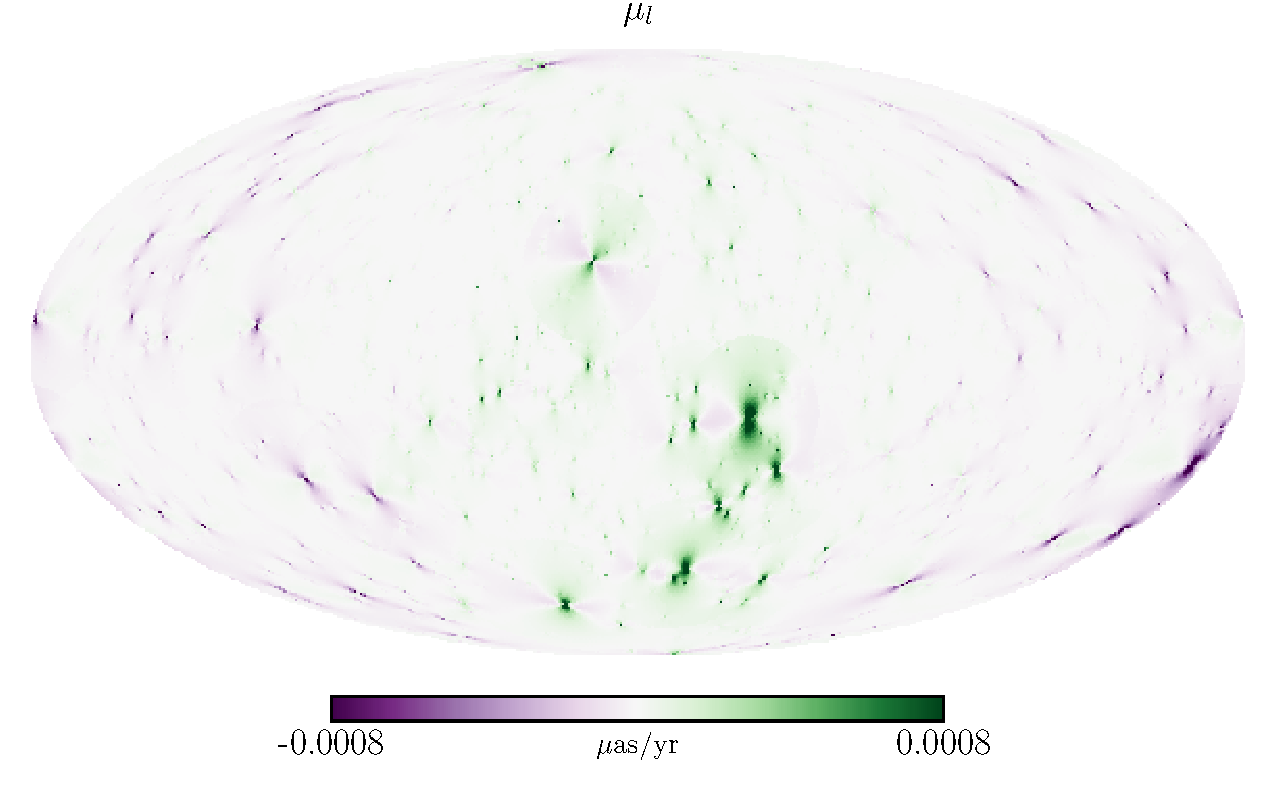
\includegraphics[width=0.45\textwidth]{plots/mu_l}
  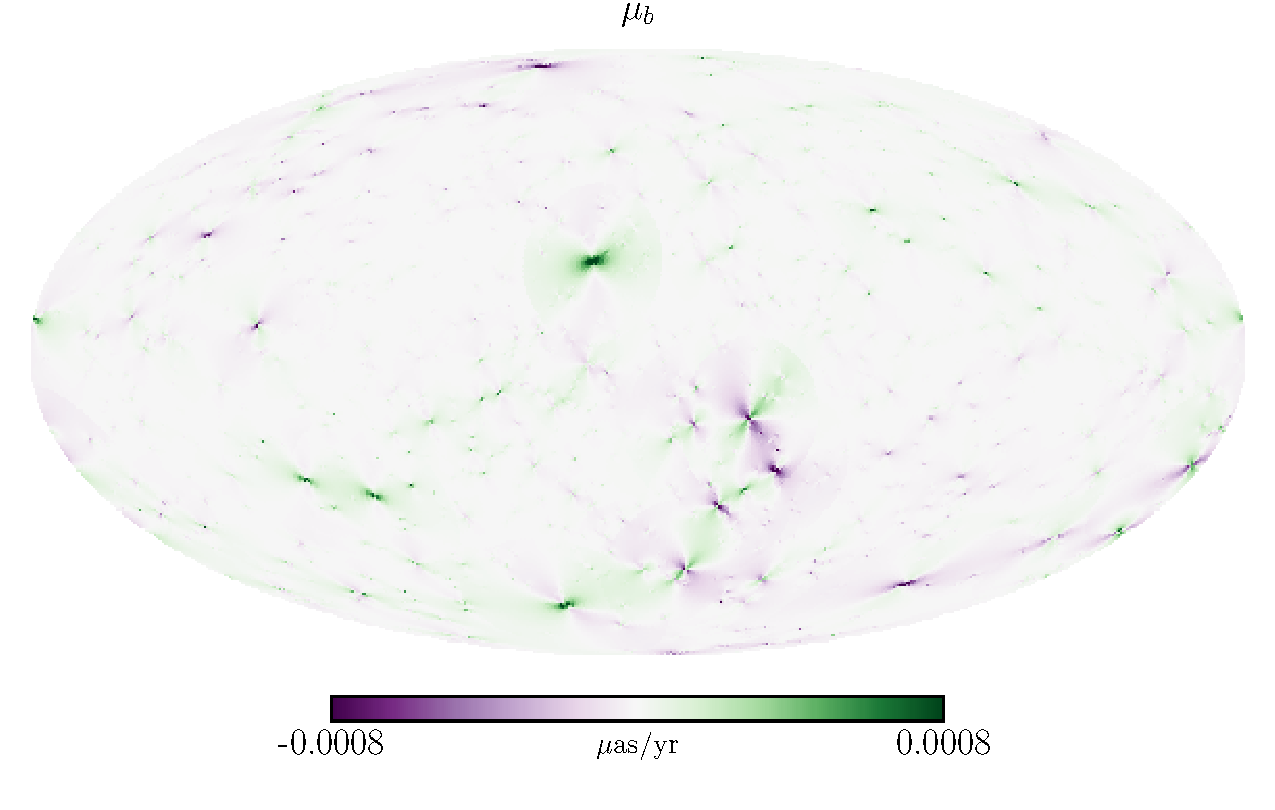
\includegraphics[width=0.45\textwidth]{plots/mu_b}
  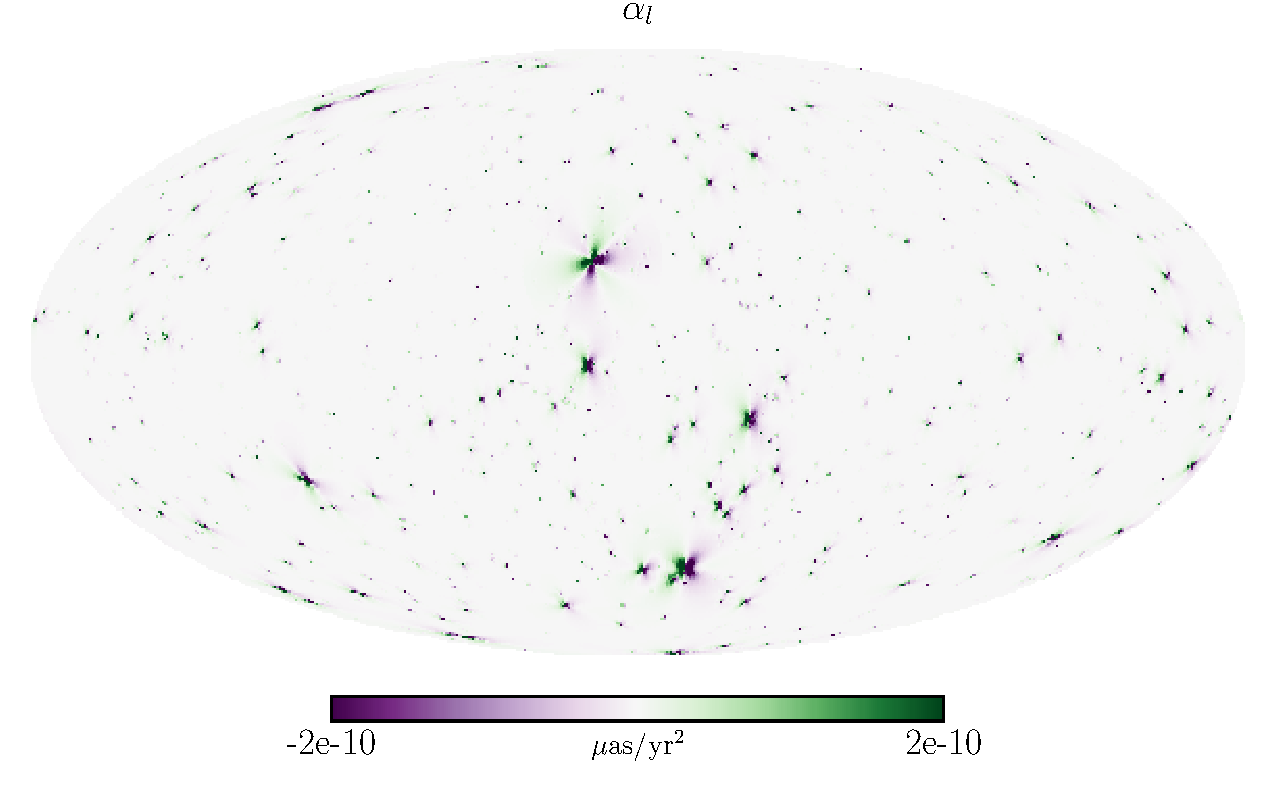
\includegraphics[width=0.45\textwidth]{plots/alpha_l}
  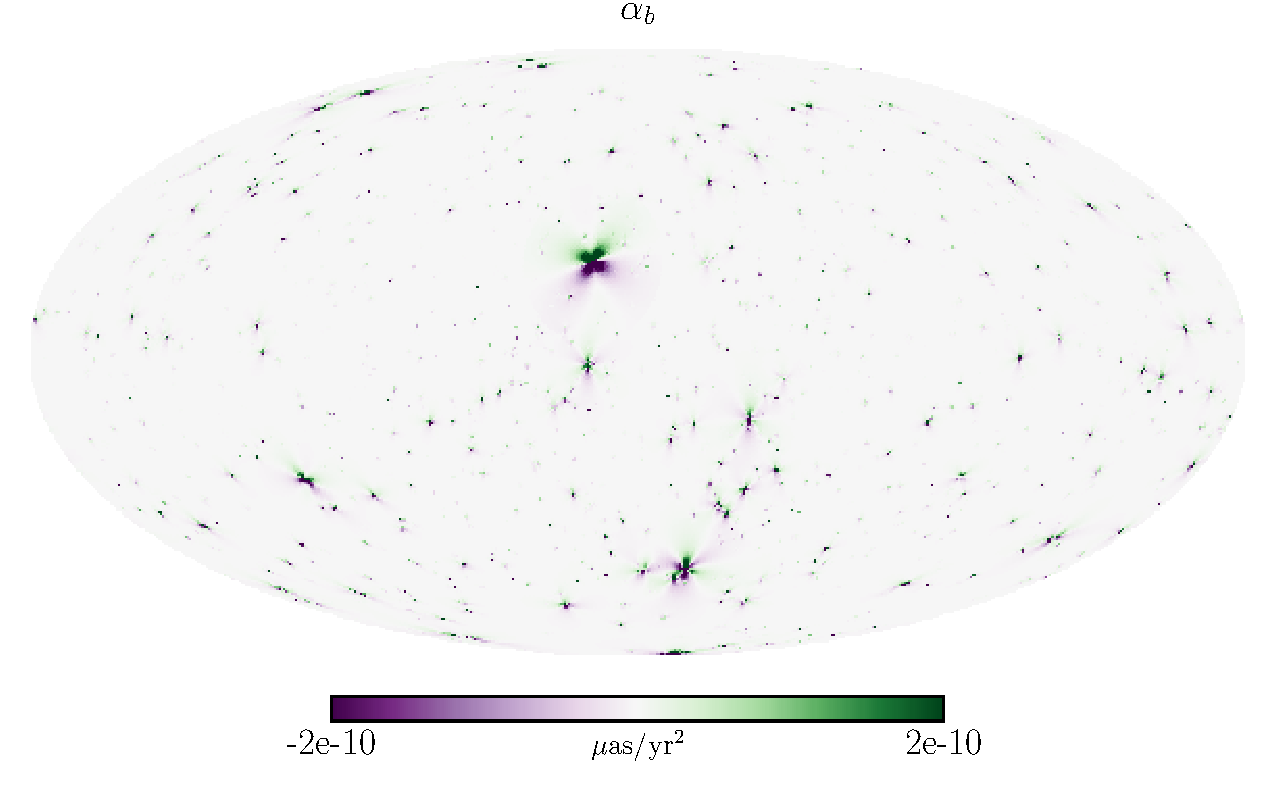
\includegraphics[width=0.45\textwidth]{plots/alpha_b}
  \caption{Proper motion (top row) and proper motion acceleration (bottom row) induced by a simulated realization of subhalos using the CDM-inspired fiducial configuration. Galactic longitude (left column) and Galactic latitude (right column) components are shown on a \texttt{HEALPIX} grid with resolution \texttt{nside} = 128.}
  \label{fig:population_maps}
\end{figure*}


\section{Formalism and warm-up}
\label{sec:singlesh}

Our goal is to compute the two-point correlation function of lens-induced velocities and accelerations due to a population of Galactic subhalos. In this section, we provide an overview of this formalism, leaving details of the derivations to App.~\ref{app:derivations}. We then apply this formalism to a few simple subhalo populations to build intuition for how the signal characteristics are affected by the properties of the underlying substructure population.

\subsection{Vector power spectrum formalism}
\label{sec:formalism}

\subsubsection*{Lens-induced proper motions and accelerations}

In the thin-lens regime, the angular deflection $\Delta \boldsymbol{\theta}$ of a source at angular diameter distance $D_s$ due to a lens at angular diameter distance $D_l$ is~(see \emph{e.g.}, V18)
\begin{equation}
\Delta \boldsymbol{\theta}=-\left(1-\frac{D_{l}}{D_{s}}\right) \frac{4 G_{N} M(b)}{b} \hat{\mathbf{b}}
\end{equation}
where $\vect{b}$ is the physical impact parameter between the source and lens, and $M(b)$ is the enclosed mass function of the spherically-symmetric lens within a cylinder of radius $b$, $M\left(b\right)=2 \pi \int_{-\infty}^{+\infty} \mathrm{d} x \int_{0}^{b} \mathrm{d} b^{\prime} b^{\prime} \rho\left(\sqrt{x^{2}+b^{\prime 2}}\right)$. As discussed in V18, the induced deflections are typically too small to be disentangled from naturally-occurring and systematic variations in the angular number density of sources, either individually or collectively.

Time-domain effects offer more promise. Since dark matter substructure has a characteristic velocity dispersion, an effective lens velocity $\vect{v}_l \equiv {\dd \vect{b}}/{\dd t}$ induces an apparent velocity on the luminous sources. This angular velocity correction $\vect{\mu}\equiv\Delta\boldsymbol{\dot \theta}$ can be written as 
\begin{align}
\vect{\mu}(\vect{b}) = 4 G_N \left\lbrace \frac{M(b)}{b^2} \left[ 2 \hat{\vect{b}} (\hat{\vect{b}} \cdot \vect{v}_l) -  \vect{v}_l \right] -\frac{M'(b)}{b} \hat{\vect{b}} (\hat{\vect{b}} \cdot \vect{v}_l) \right\rbrace.
\label{eq:mureal}
\end{align}
We will often use the angular separation $\vect{\beta} \equiv \vect{b}/D_l = \vect{\theta}_l -  \vect{\theta}_s$  between celestial positions of the lens and source, $\vect{\theta}_l$ and $\vect{\theta}_s$, respectively. 
In Eq.~\ref{eq:mureal} above, we have ignored a $(1-{D_l}/{D_s})$ geometric factor in the limit of large source distance $D_s$ relative to the line-of-sight distance $D_l$ to the lens. Equation~\ref{eq:mureal} represents a dipole pattern centered at the lens position, which can be seen the top row of Fig.~\ref{fig:population_maps}.

The induced acceleration can be calculated similarly by taking an additional derivative of Eq.~\ref{eq:mureal} (see V18 for details). This results in a quadrupole pattern centered on the lens position, which can be seen the bottom row of Fig.~\ref{fig:population_maps}. Induced acceleration are suppressed by characteristic factors of $\sim v_l/b$ compared to induced velocities. 

A key feature of induced velocities vs accelerations can be seen in Fig.~\ref{fig:population_maps} --- while the velocity signal is dominated by the heaviest objects, the acceleration signal is much more democratic and is preferentially sensitive to a population of dense, low-mass subhalos.

\subsubsection*{Vector spherical harmonic decomposition}

The power spectrum decomposition of vector fields on a sphere (\emph{e.g.}, in our case the proper motions and accelerations measured over some fraction of the sky) relies on the vector spherical harmonic (VSH) decomposition, which is an extension of the scalar spherical harmonic decomposition ubiquitous in astrophysics and cosmology. In particular, given a vector field $\vect \mu = \vect \mu(\vect \theta)$ on sphere, this admits a multipole expansion
\begin{align}
\vect{\mu} = \sum_{\ell m} \mu^{(1)}_{\ell m} \vect{\Psi}_{\ell m} + \mu^{(2)}_{\ell m} \vect{\Phi}_{\ell m},
\label{eq:vsh_decomposition}
\end{align}
with poloidal ($\vect{\Psi}$) and toroidal ($\vect{\Phi}$) amplitudes 
\begin{align}
\mu^{(1)}_{\ell m} =  \int \dd \Omega \, \vect{\mu} \cdot \vect{\Psi}^*_{\ell m};\quad
 \mu^{(2)}_{\ell m} =  \int \dd \Omega \, \vect{\mu} \cdot \vect{\Phi}^*_{\ell m},
 \label{eq:harmdecomposition}
\end{align}
where the vector spherical harmonics (VSH) are defined as
\begin{align}
\vect{\Psi}_{\ell m} = \frac{\vect{\nabla}_{\vect{\theta}} Y_{\ell m}}{\sqrt{l(l+1)}}; \quad \vect{\Phi}_{\ell m} = \hat{\vect{r}} \times 
\vect{\Psi}_{\ell m} \label{eq:PsiPhidef}
\end{align}
in spherical coordinates $\lbrace r, \theta, \phi \rbrace$ with $\theta$ and $\phi$ Galactic colatitude and longitude respectively (sometimes combined in the 2D vector $\vect{\theta} = \lbrace \theta, \phi \rbrace$ with corresponding angular gradient $\vect{\nabla}_{\vect{\theta}}$), and $r$ the radial, line-of-sight direction. The above VSH are normalized such that they are orthonormal on the sphere $\int \dd \Omega \, \vect{V}_{\ell m} \cdot \vect{V}_{\ell' m'}  = \delta_{\vect{V}'\vect{V}} \delta_{\ell' \ell} \delta_{m' m}$ with $\vect{V} = \{\vect{\Psi},\vect{\Phi}\}$, and form a complete basis for a vector field on the celestial sphere. The power-per-mode can be then obtained as usual as 
\begin{equation}
C_{\ell}^{\mu} \equiv \frac{1}{2\ell + 1} \sum_{m = -\ell}^{\ell} \left| \mu_{\ell m} \right|^2.
\end{equation}

Physically, Eq.~\ref{eq:vsh_decomposition} corresponds to decomposing a vector field into a \emph{curl-free} component (the first term, also known as poloidal), which can be written as the gradient of a sourcing scalar potential, and a \emph{divergence-free} component (the second term, also known as toroidal), which can be written as the curl of a sourcing vector potential. 

Application of the vector spherical harmonic decomposition formalism to lens-induced observables is straightforward. Since the lensing deflection can be written as the gradient of an effective projected (scalar) lensing potential $\psi$, $\Delta\theta \sim \vect{\nabla}_{\vect{\theta}} \psi$, it follows that the angular deflection field, and in fact \emph{all} lensing observables, only have overlap with poloidal power spectrum modes. This can be seen explicitly for the lens-induced angular velocity correction of Eq.~\ref{eq:mureal}, which can be written as
\begin{align}
 \vect{\mu} =  \frac{\dd}{\dd t} \vect{\nabla}_{\vect{\theta}} \psi = - \frac{1}{D_l} \vect{\nabla}_{\vect{\theta}} \left(\vect{v} \cdot \vect{\nabla}_{\vect{\theta}} \psi \right) \label{eq:deflectionpotential}.
\end{align} 
We therefore immediately have that $\mu_{\ell m}^{(2)}$, and the corresponding power-per-mode $C_{\ell}^{\mu (2)}$, are identically zero after integrating by parts in Eq.~\ref{eq:harmdecomposition} and noting that $\vect{\nabla}_{\vect{\theta}} \cdot \vect{\Phi}_{\ell m} = 0$.

The power-per-mode, per lens for a uniformly distributed population of lenses can be calculated once the lens properties (effective velocity, density profile and angular diameter distance) are specified (see App.~\ref{app:derivations} for derivations and details):
\begin{align}
C_{\ell}^{\mu (1)} &\equiv \frac{1}{2\ell + 1} \sum_{m = -\ell}^{\ell} \left| \mu_{\ell m}^{(1)} \right|^2 \nonumber \\
&\simeq \sum_l \left(\frac{4 G_N v_l}{D_l^2}\right)^2 \frac{\pi}{2} \ell^2 \left[\int_0^\infty \dd \beta M(\beta D_l) J_1(\ell \beta) \right]^2, \label{eq:pspec_mu}
\end{align}
where the sum over $l$ is a sum over different lenses, which can in general have different $D_l$, $v_l$, and enclosed mass functions $M(b)$.

The acceleration power spectrum can be worked out similarly and is compactly expressed in terms of the velocity power spectrum (see App.~\ref{app:derivations} for derivation): 
\begin{align}
C_{\ell}^{\alpha (1)} &\equiv \frac{1}{2\ell + 1} \sum_{m = -\ell}^{\ell} \left| \alpha_{\ell m}^{(1)} \right|^2 = \frac{3}{4} \frac{\ell^2 v_l^2}{D_l^2}\,C_{\ell}^{\mu (1)}.
\label{eq:pspec_alpha}
\end{align}
% \blue{note the factor of 3/4 instead of 3/64}

\begin{figure*}[htbp]
  \centering
  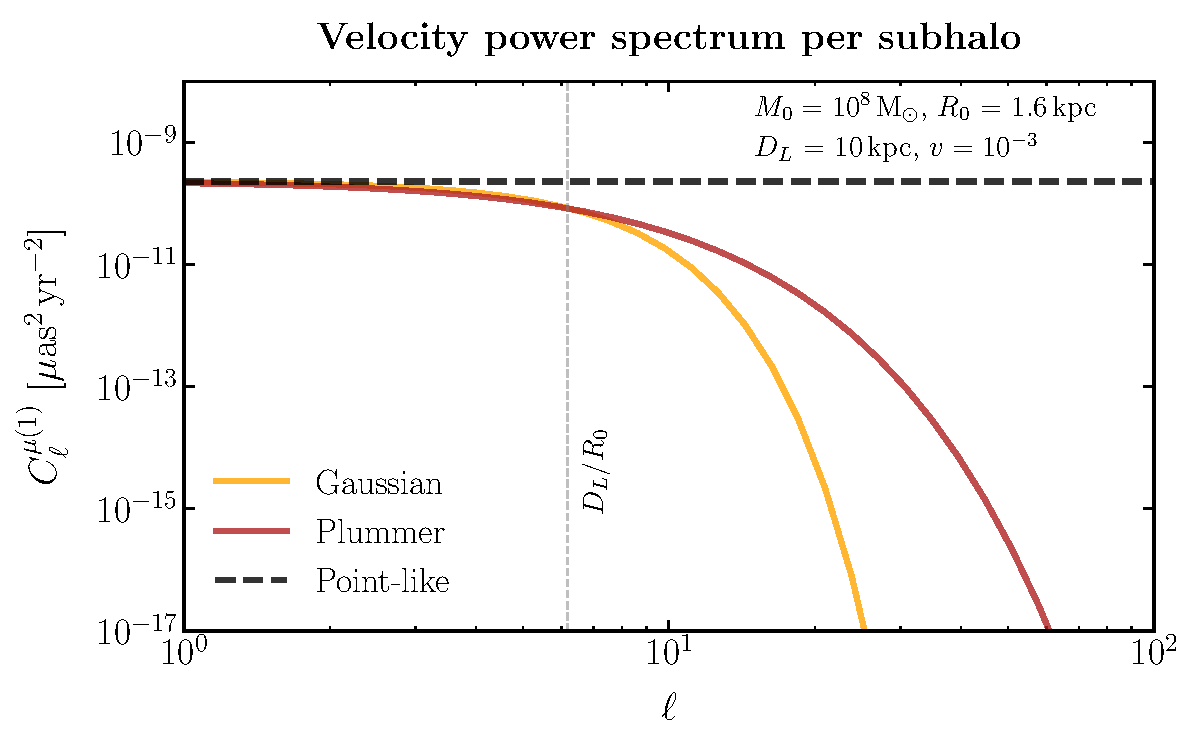
\includegraphics[width=0.45\textwidth]{plots/mu_single_1}
  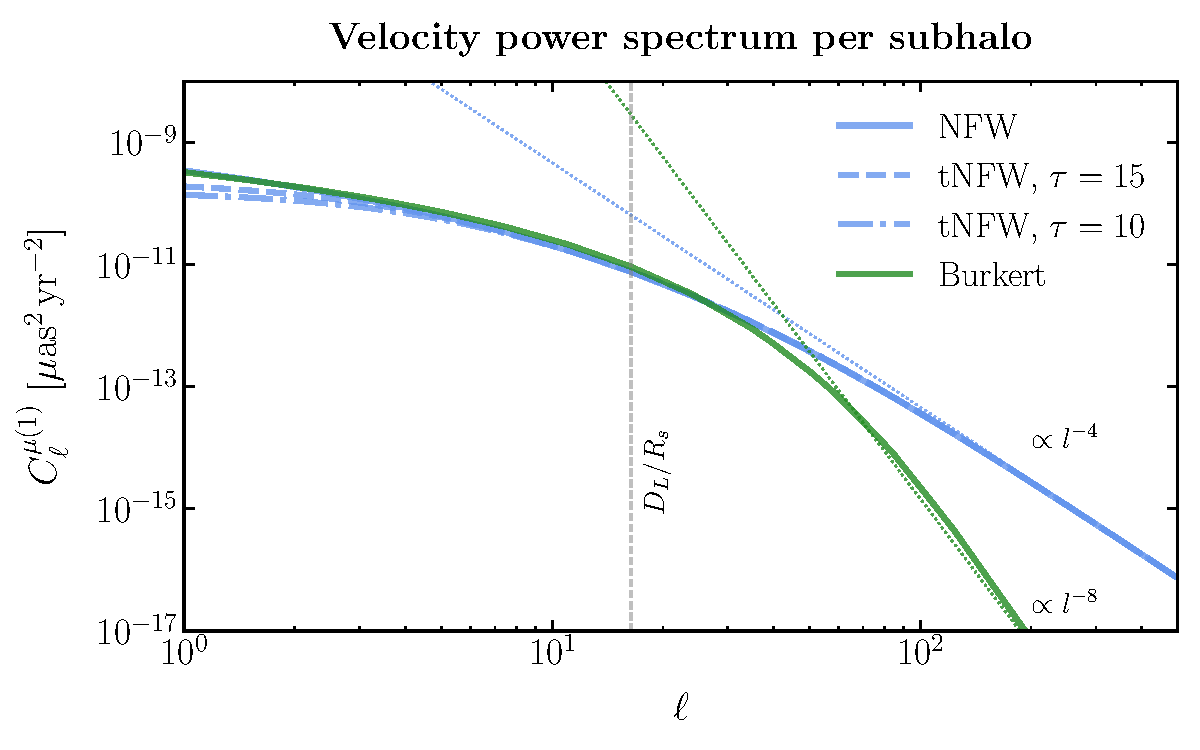
\includegraphics[width=0.45\textwidth]{plots/mu_single_2}
  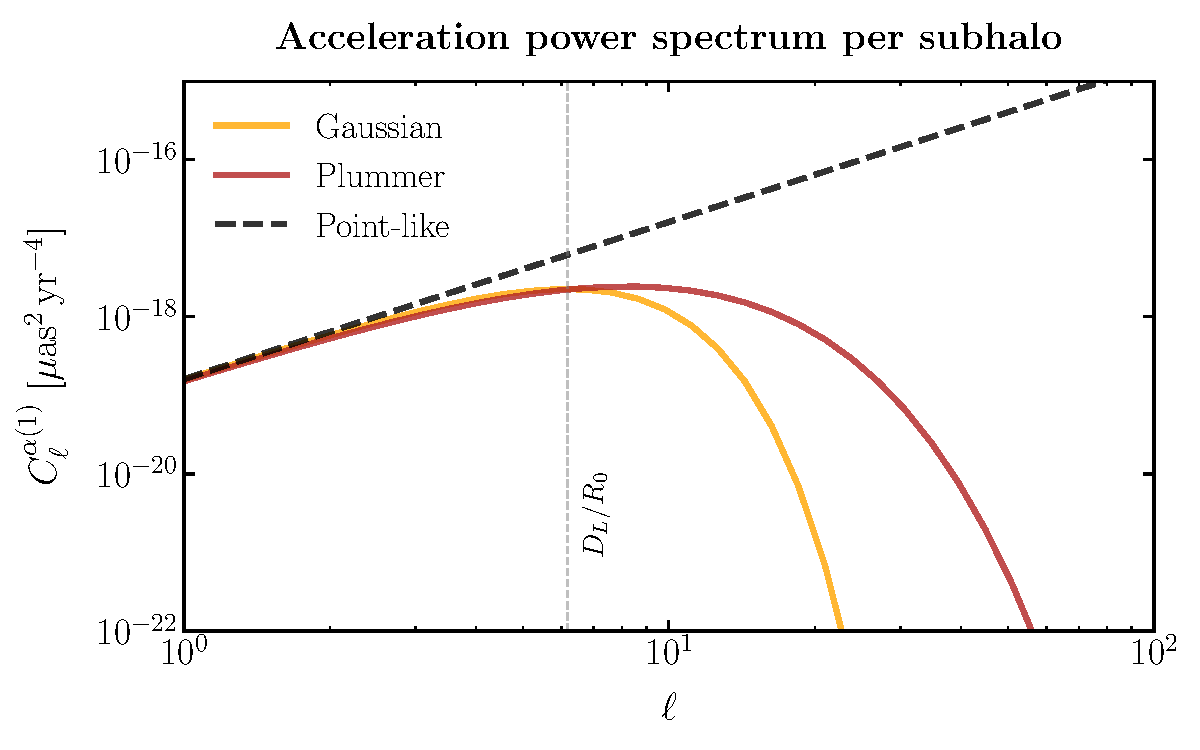
\includegraphics[width=0.45\textwidth]{plots/alpha_single_1}
  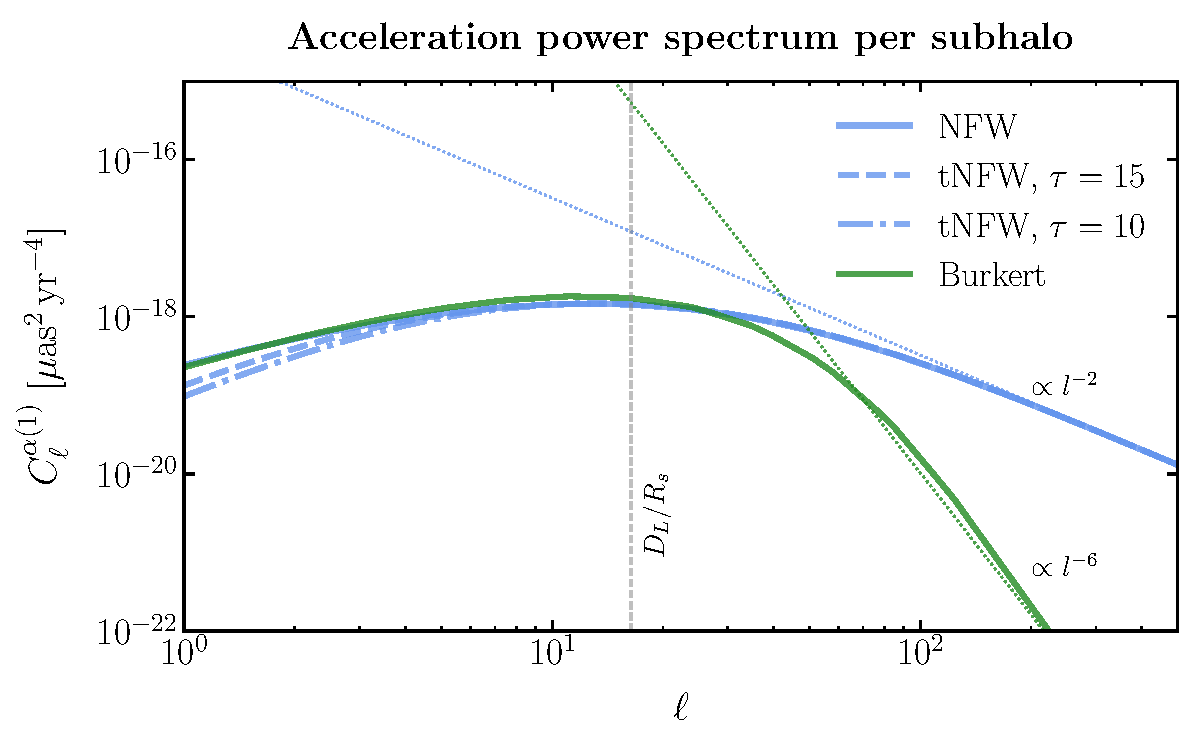
\includegraphics[width=0.45\textwidth]{plots/alpha_single_2}
  \caption{Expected lens-induced proper motion (top row) and proper motion acceleration (bottom row) power spectra per subhalo for a homogeneous subhalo population. Shown for Gaussian and Plummer profiles (left column) with $M_0 = 10^{8}$\,M$_\odot$, $D_l=10$\,kpc, $R_0=1.6$\,kpc and $v_l=10^{-3}$ as well as NFW, two different truncated NFW ($\tau \equiv r_t/r_s = 10, 15$) and Burkert profiles (right column) with $M_{200}=10^{8}$\,M$_\odot$, $c_{200}=5$, $D_l=10$\,kpc and $v_l=10^{-3}$. High-$\ell$ asymptotic behavior for the NFW and Burkert profiles is shown.} 
  \label{fig:single_sub}
\end{figure*}

\subsection{Warm-up and examples}
\label{sec:examples}

Once the subhalo properties (enclosed mass function, distance and transverse velocity) have been specified, the lens-induced proper motion and proper motion acceleration signal power spectra can readily be calculated from Eqs.~\ref{eq:pspec_mu} and~\ref{eq:pspec_alpha}. We illustrate this for a few specific cases, starting from simple scenarios and going to progressively more realistic ones, in order to gain some intuition for how the signal significance depends on properties of the subhalo population, as well as which multipoles $\ell$ contribute to the signal in various cases. Unless otherwise specified, all spectra refer to the respective poloidal components $C_{\ell}^{\mu/\alpha (1)}$, with the toroidal signal components $C_{\ell}^{\mu/\alpha (2)}$ identically vanishing (cf. Eq.~\ref{eq:deflectionpotential}). In the interest of conciseness, we summarize the main takeaways of this section at the end in Sec.~\ref{sec:summary},

We appeal to the Fisher information formalism to isolate and study the contribution of different multipoles in a power spectrum measurement (See App.~\ref{sec:fisher} for details). For a given signal $C_{\ell}^{\mu (1)}$ and noise $N_{\ell}^{\mu}$ configuration, the Fisher information contained in a mode $\ell$ simplifies to (Eq.~\ref{eq:fisher}) 
\begin{equation}
F_\ell = f_\mathrm{sky}(\ell + 1/2) \left(\frac{C_{\ell}^{\mu (1)}}{C_{\ell}^{\mu (1)} + N_{\ell}^{\mu}}\right)^2
\label{eq:fisher_l}
\end{equation}
where $f_\mathrm{sky}$ is the fraction of the sky over which the measurement is made. Formally, the Fisher information corresponds to the inverse of the minimum possible variance with which a measurement can be made, and quantifies the information extractable from each mode.

The noise power spectrum is scale-invariant and is approximately given by
\begin{equation}
N_{\ell}^{\mu/\alpha} \simeq \frac{4\pi\sigma_{\mu/\alpha}^2}{N_q}
\end{equation}
where $\sigma_{\mu/\alpha}$ is the measurement error on the proper motions or accelerations and $N_q$ the number of objects (\emph{e.g.}, quasars or stars) sampled, assumed uniform over the full sky. Note that for a partial-sky measurement, both the signal and noise scale the same way (proportional to $f_\mathrm{sky}$), and the information loss comes from the mode multiplicity pre-factor in Eq.~\ref{eq:fisher_l}.

For a power spectrum measurement of multipoles between $[\ell_\mathrm{min}, \ell_\mathrm{max}]$ the significance of a given signal is given by the square root of the inverse covariance, and with each mode constituting an independent measurement can be computed from the Fisher information as
\begin{equation}
\sigma_\mathrm{sig}\equiv\mathrm{Cov}^{-1/2}=\sqrt{\sum_{\ell = \ell_\mathrm{min}}^{\ell_\mathrm{max}}F_\ell}.
\label{eq:signif}
\end{equation}
Thus, $F_\ell$ quantifies the contribution of each mode to the total signal significance. We illustrate this for a few toy examples to gain some intuition for the various relevant scales in the problem.

\subsubsection{Population of point lenses}

We start by considering a population of points lenses of mass $M_0$ located at a given distance $D_l$. In this case, the power per mode per lens is given by (Eq.~\ref{eq:pspec_mu})
\begin{equation}
C_{\ell}^{\mu (1)} \simeq \left(\frac{4 G_N M_0 v}{D_l^2}\right)^2 \frac{\pi}{2}.
\end{equation}
This scale-invariant spectrum is shown on the top left plot of Fig.~\ref{fig:single_sub} as the dotted black line, for the lens population properties in the inset.

For a population isotropically distributed between $D_l^{\mathrm{min}}$ and $D_l^{\mathrm{max}}$ and making up a fraction $\Omega_l$ of the local dark matter density $\rho_\mathrm{DM}$, we have
\begin{equation}
C_{\ell}^{\mu (1)} \simeq \frac{32 \pi^{2} G_{\mathrm{N}}^{2} M_{0} \Omega_{l} \rho_{\mathrm{dm}} v^{2}\left(D_{l}^{\mathrm{max}}-D_{l}^{\mathrm{min}}\right)}{D_{l}^{\mathrm{max}} D_{l}^{\mathrm{min}}}
\label{eq:mu_pspop}
\end{equation}

For a point lens population, the proper motion power per mode is scale-invariant, with higher modes having greater mode multiplicity. Hence, the Fisher information per mode grows as $F_\ell^\mu\sim \sqrt{\ell}$, with the total significant growing linearly with maximum multiple probed $\sigma_\mathrm{sig}^\mu\propto\ell_\mathrm{max}$ in the noise-dominated ($N_\ell^\mu\gg C_{\ell}^{\mu (1)}$) regime. Of course, in practice the maximum possible multipole $\ell_\mathrm{max}$ is limited by telescope resolution and pixelization effects, as well as shot noise due to finite source density.

The acceleration power spectrum can be calculated similarly using Eq.~\ref{eq:pspec_alpha} and shown in the bottom left plot of Fig.~\ref{fig:single_sub} as the dotted black line for the lens properties in the inset text. Unlike the velocity power spectrum, it is not scale-invariant, and the significance with increasing maximum multipole $\ell_\mathrm{max}$ grows approximately as $\sigma_\mathrm{sig}^\alpha\propto\ell_\mathrm{max}^3$. Thus, the acceleration power spectrum preferentially probes smaller scales compared to the proper motion power spectrum. 

\begin{figure}[htbp]
  \centering
  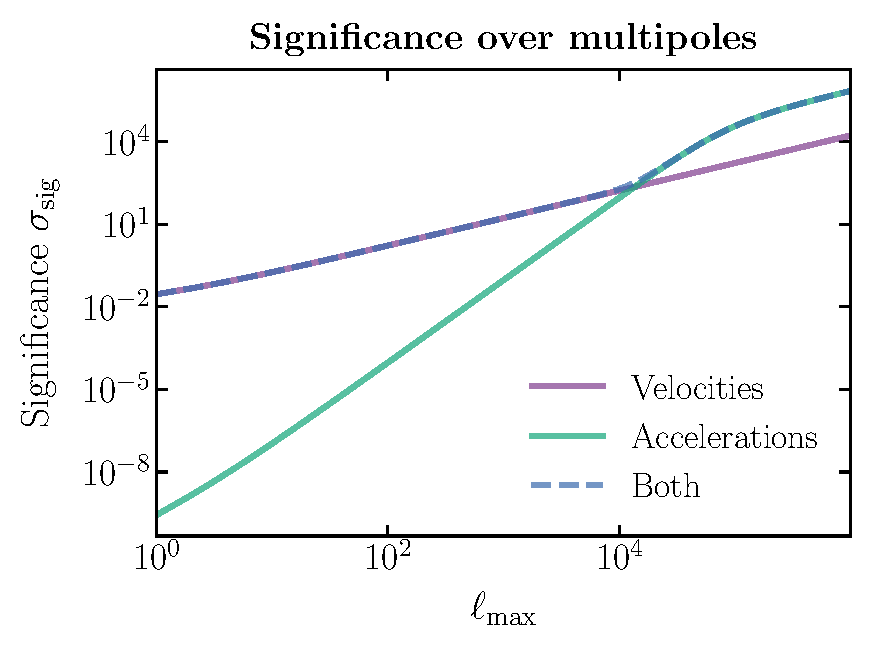
\includegraphics[width=0.45\textwidth]{plots/mualpha_compact}
  \caption{Signal significance as a function of maximum multipole $\ell_\mathrm{max}$ probed, shown for a population of $M_0=10^8$\,M$_\odot$ point source lenses uniformly distributed between $D_l^{\mathrm{min}}=0.1$\,kpc and $D_l^{\mathrm{max}}=10$\,kpc making up all of the local dark matter density $\rho_\mathrm{DM}=0.4$\,GeV\,cm$^{-3}$ with $v_l=10^{-3}$. $N_q=10^8 (10^{11})$ background sources with measurement errors $\sigma_\mu=100\,\mu$as\,yr$^{-1}$ ($\sigma_\alpha=10\,\mu$as\,yr$^{-2}$) are assumed for proper motion and acceleration measurement. Shown are the contributions from the proper motion power spectrum (purple), proper motion acceleration power spectrum (green) and both (dotted blue). The acceleration power spectrum probes smaller scales and smaller distances.} 
  \label{fig:mualpha_compact}
\end{figure}

Figure~\ref{fig:mualpha_compact} illustrates the detection significance as a function of maximum multipole $\ell_\mathrm{max}$, as defined in Eq.~\ref{eq:signif}, for a population of $M_0=10^8$\,M$_\odot$ point source lenses uniformly distributed between $D_l^{\mathrm{min}}=0.1$\,kpc and $D_l^{\mathrm{max}}=10$\,kpc making up all of the local dark matter density $\rho_\mathrm{DM}=0.4$\,GeV\,cm$^{-3}$. $N_q=10^8 (10^{11})$ background sources with measurement errors $\sigma_\mu=100\,\mu$as\,yr$^{-1}$ ($\sigma_\alpha=10\,\mu$as\,yr$^{-2}$) are assumed for proper motion(acceleration) measurements, for illustration. At higher multipoles $\ell_\mathrm{max}\gtrsim10^4$, the acceleration power spectrum provides the dominant contribution in this case. The exact crossover point is sensitive to characteristic distance of the nearest sources $D_{l}^{\mathrm{min}}$, since the significance in either case is most sensitive to nearby sources, and the acceleration power spectrum scales more favorably with lower $D_{l}$ compared to the velocity power spectrum. For a general lens distribution, the smaller the typical distance that contributes to the total power, the greater the relative importance of accelerations. Its relative importance also grows with integration time $\tau$, since typically $\sigma_\alpha/\sigma_\mu\sim1/\tau^2$. These arguments naturally carry over to the case of extended lenses, which we consider next.

\subsubsection{Population of extended lenses}
\label{sec:extended_pop}

\begin{figure*}[htbp]
  \centering
  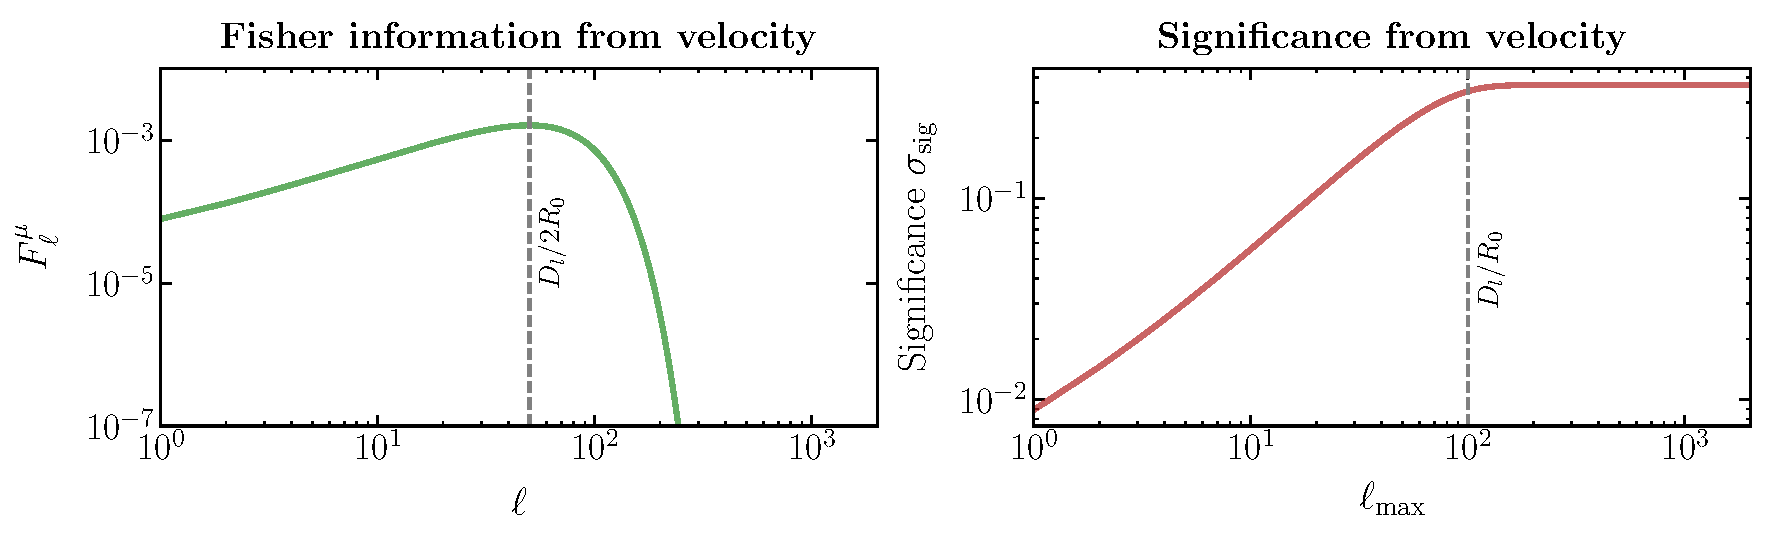
\includegraphics[width=0.9\textwidth]{plots/fisher_mu_single}
  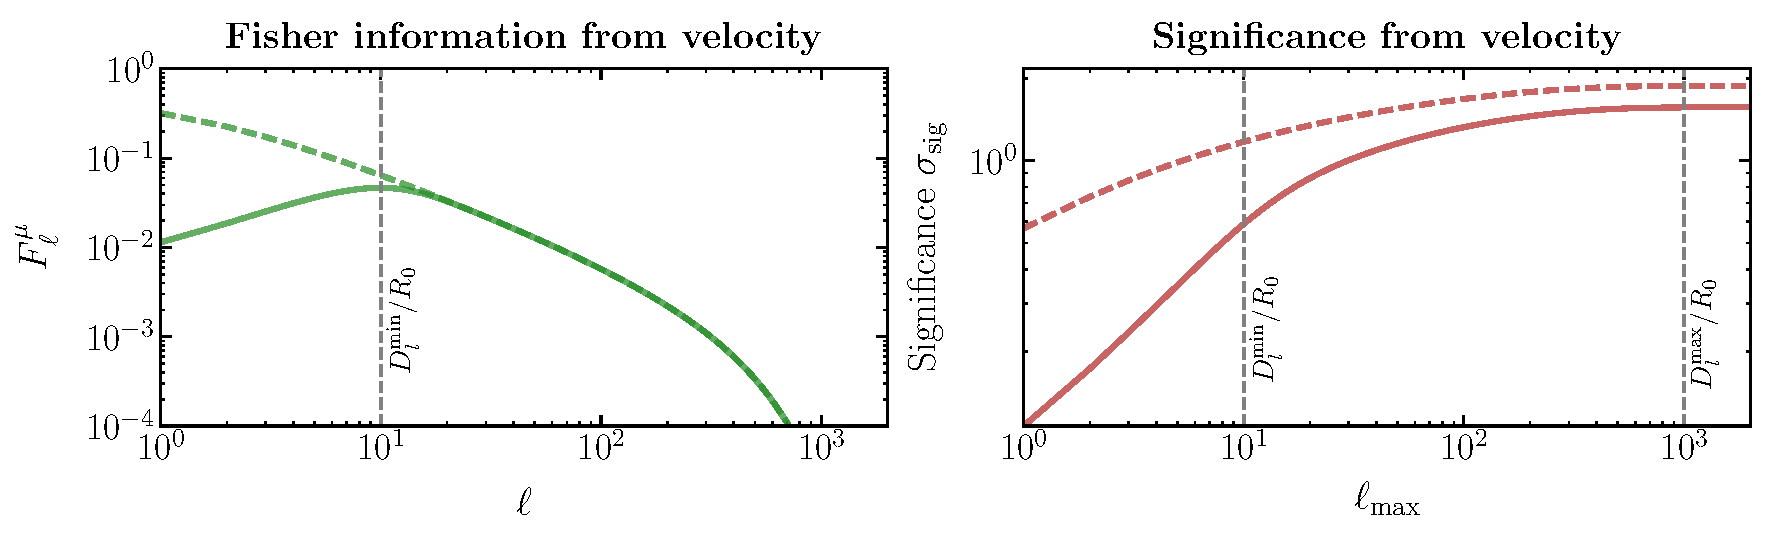
\includegraphics[width=0.9\textwidth]{plots/fisher_mu}
  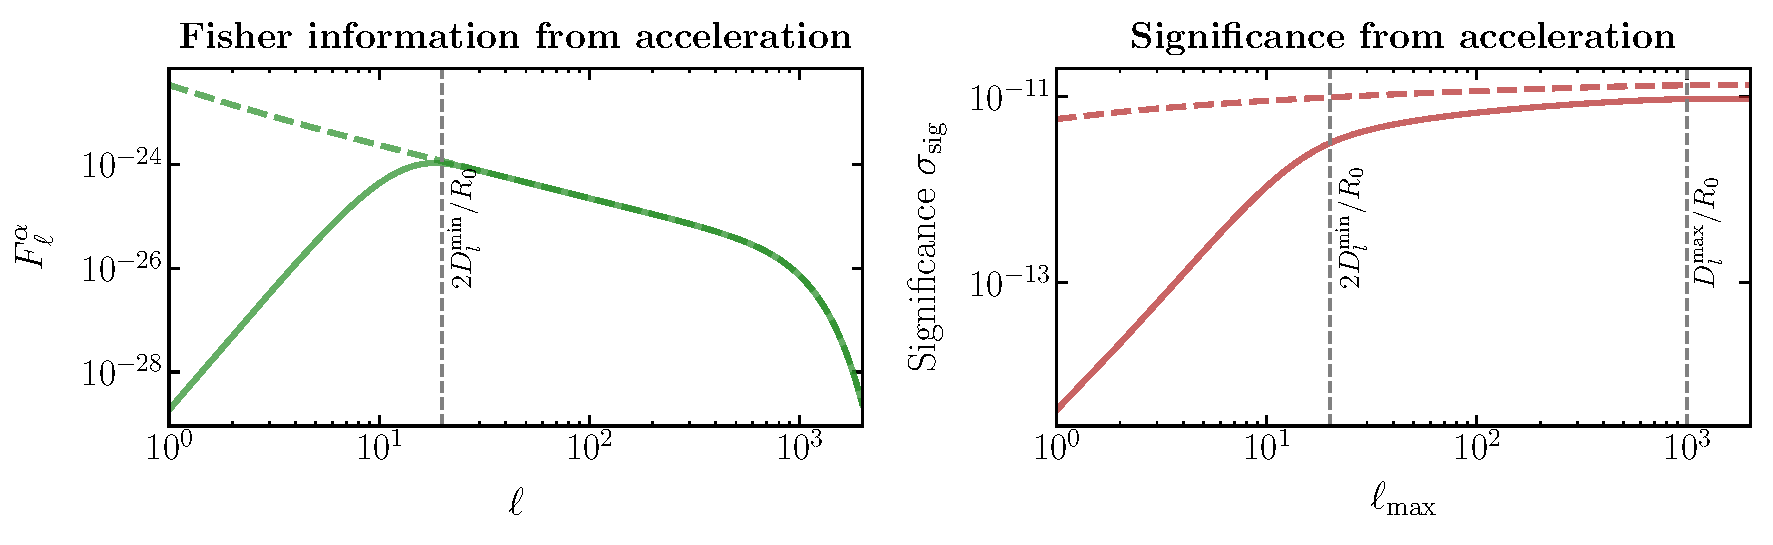
\includegraphics[width=0.9\textwidth]{plots/fisher_alpha}
  \caption{Fisher information (left column) and significance (right column), as defined in Eq.~\ref{eq:fisher_l} and Eq.~\ref{eq:signif} respectively, for Gaussian lenses at equal-distance $D_l=1\,\mathrm{kpc}$ (top row, from velocity power spectra), a population between $D_{l}^{\mathrm{min}}=0.1\,\mathrm{kpc}$ and $D_{l}^{\mathrm{max}}=10\,\mathrm{kpc}$ (middle and bottom row, from velocity and acceleration power spectra respectively). The same population parameters as in Fig.~\ref{fig:mualpha_compact} are assumed, with spatially extended lenses extension $R_0=10$\,pc. Dotted lines correspond to taking $D_l^\mathrm{min}=0$. Measurement errors $\sigma_\mu=50\,\mu$as\,yr$^{-1}$ and $\sigma_\alpha=5\,\mu$as\,yr$^{-2}$ are assumed.} 
  \label{fig:fisher_sig}
\end{figure*}

In order to motivate the study of spatially extended subhalos and understand how the lensing power spectrum signal depends on the nature of extension, we consider a population of Gaussian lenses with density profile 
\begin{equation}
\rho(r) =\frac{M_0}{2\sqrt{2}\pi^{3/2}R_0^3} e^{-r^2/2R_0^2} 
\label{eq:Gaussianrho}
\end{equation} 
where $M_0$ is the total lens mass and $R_0$ its characteristic size. The integral in Eq.~\ref{eq:pspec_mu} can be carried out analytically, yielding
\begin{equation}
C_{\ell}^{\mu (1)} \simeq \left(\frac{4 G_N M_0 v}{D_l^2}\right)^2 \frac{\pi}{2} e^{-\ell^2\beta_0^2}
 \label{eq:mu_ext}
\end{equation}
where $D_l$ is distance to the lens and $\beta_0 \equiv R_0/D_l$ the characteristic angular scale. The power spectrum per lens is shown in the top left plot in Fig.~\ref{fig:single_sub} as the yellow line, and falls off exponentially with characteristic scale $\ell \sim D_l/R_0$.

The Fisher information and significance in this case is illustrated on the left and right of the top row of Fig.~\ref{fig:fisher_sig}, respectively. The same lens properties are assumed as for Fig.~\ref{fig:mualpha_compact}, with lens size $R_0=10$\,pc and lenses at $D_l=1$\,kpc, assuming noise properties $\sigma_\mu = 50\,\mu\mathrm{as}\,\mathrm{yr}^{-1}$ and $N_q = 10^8$. The maximum Fisher information is contained at scales $\ell \approx {D_l}/{2R_0}$, with the significance growing linearly with $\ell_\mathrm{max}$ until $\ell \approx {D_l}/{R_0}$ when it plateaus and there is little information in higher modes. 

This gives us some intuition for the more realistic case of a population of such lenses distributed between $D_l^{\mathrm{min}}$ and $D_l^{\mathrm{max}}$. Here, we have the power per mode 
\begin{align}
C_{\ell}^{\mu (1)} \simeq 16 \pi ^{5/2} &G_\mathrm{N}^2 M_0 \rho_\mathrm{DM} v^2 \Omega_l\times\nonumber\\ &\left[\frac{{\mathrm{erf}}\left(\frac{\ell
   {R_0}}{D_l^{\mathrm{min}}}\right)-{\mathrm{erf}}\left(\frac{\ell {R_0}}{{D_l^{\mathrm{max}}}}\right)}{\ell {R_0}}\right].
 \label{eq:mu_extpop}
\end{align}

The Fisher information and significance over different modes for this case are shown in the middle panel of Fig.~\ref{fig:fisher_sig}. The same lens properties are assumed as for Fig.~\ref{fig:mualpha_compact}, with lens size $R_0=10$\,pc, assuming noise properties $\sigma_\mu = 50\,\mu\mathrm{as}\,\mathrm{yr}^{-1}$ and $N_q = 10^8$. In the noise-dominated regime, the Fisher information for this population peaks at $\ell \sim D_l^{\mathrm{min}}/R_0$, insensitive to other lens properties. The growth in significance until this point is again roughly linear. Since in the case when all lenses are at the same distance the peak is at $\ell \sim D_l/(2 R_0)$, this is already indicative that $\mathcal{O}(1)$ of the total power comes from the nearest lenses. Multipoles $\ell > D_l^{\mathrm{min}}/R_0$ contribute only logarithmically to the total significance, with a cutoff around $\ell \sim D_l^{\mathrm{max}}/R_0$ where the significance plateaus. 

A similar story holds for accelerations. The power spectrum per lens is shown as the yellow line in the bottom left of Fig.~\ref{fig:single_sub}. The Fisher information per mode and cumulative significance are shown in the bottom row of Fig.~\ref{fig:fisher_sig}, assuming $\sigma_\alpha = 5\,\mu\mathrm{as}\,\mathrm{yr}^{-2}$ and everything else the same as before. Higher multipoles (smaller scales) contribute preferentially as compared to to velocity power spectra, with the maximum information coming from multipoles $\ell \sim 2D_l^{\mathrm{min}}/R_0$, and the significance flattening out at $\ell \sim 2D_l^{\mathrm{max}}/R_0$. Note the relative normalization between the velocity and acceleration cases --- although the significance with $\ell_\mathrm{max}$ for acceleration grows faster than for velocity, the lens extension effectively suppresses the former contribution, unlike in the case of point lenses where accelerations can dominate at high multipoles. A larger relative background source density is needed to leverage acceleration spectra, accessing higher multipoles where the acceleration spectra can be useful for more compact lenses.

% To summarize, $\mathcal{O}(1)$ of the power comes from $\ell < D_l^{\mathrm{min}}/R_0$, with logarithmic contribution beyond this at each $\ell$ interval, flattening out at $\ell \sim D_l^{\mathrm{max}}/R_0$.

Also unlike in the point lenses case, there is nothing preventing us from considering the limit $D_l^\mathrm{min}\rightarrow0$, since the origin singularity is regulated in the case of fluffier lenses. In this case, there is additional contribution from larger scales $\ell\lesssim D_l^\mathrm{min}$ compared to the case just considered, and there is universal logarithmic scaling of significance with $\ell_\mathrm{max}$. This is illustrated with the dotted lines for velocities (middle row) and accelerations (bottom row) in Fig.~\ref{fig:fisher_sig}.

It is instructive also to consider how the ``peak'' significance, $\sigma_\mathrm{sig}(\ell_\mathrm{max} = D_l^\mathrm{max}/R_0)$, scales with $D_l^\mathrm{max}$. This is clear from the previous section --- significance receives equal contribution per decade in $\ell_\mathrm{max}$ until $\ell_\mathrm{max} \sim D_l^\mathrm{max}/R_0$. Hence, the peak significance also receives equal contribution per logarithmic \emph{distance} interval probed.

Finally, we consider the impact of lens extension on detection significance. The significance using velocity spectra $\ell \in [10, 10^4]$ as a function of extension $R_0$ is shown in Fig.~\ref{fig:sig_R0}, for lenses located at distance $D_l$ and for $M_0 = 10^{7}(10^{8})\,\mathrm{M}_\odot$ in purple(green). Two relevant scales can be seen. The cutoff $\ell_\mathrm{max}$ means that extra power at smaller scales cannot be leveraged for lenses smaller than $R_0 \lesssim D_l/\ell_\mathrm{max}$. The cutoff $\ell_\mathrm{min}$ means that the significance falls off exponentially for lenses $R_0 \gtrsim D_l/\ell_\mathrm{min}$, where the dominant contribution comes from scales larger than the cutoff. Between these scales, significance falls of approximately linearly with lens extension. For lenses distributed uniformly between $D_l^\mathrm{min}$ and $D_l^\mathrm{max}$, this means that the significance plateaus for $R_0 \lesssim D_l^\mathrm{min}/\ell_\mathrm{max}$ and falls off rapidly for $R_0 \gtrsim D_l^\mathrm{max}/\ell_\mathrm{min}$. Note also from Fig.~\ref{fig:sig_R0} (and Eqs.~\ref{eq:mu_ext} and~\ref{eq:mu_extpop}) that the various scales of interest do not depend on the lens mass $M_0$, with the total significance scaling quadratically with $M_0$ (or linearly in the case of a uniformly distributed population of lenses).

\begin{figure}[htbp]
  \centering
  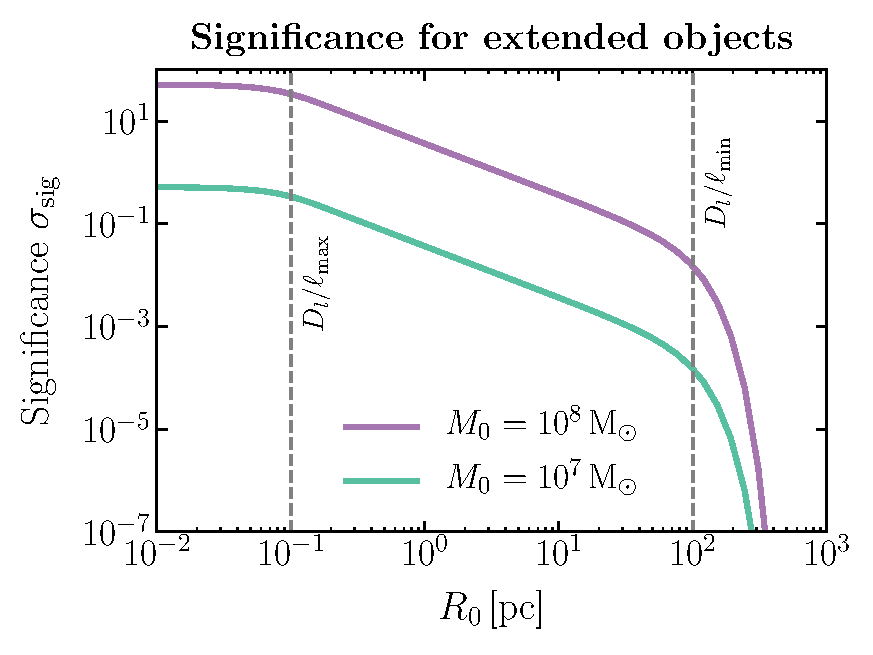
\includegraphics[width=0.45\textwidth]{plots/sig_R0}
  \caption{Detection significance as a function of spatial extension $R_0$ illustrated for Gaussian lenses at distance $D_l=10\,\mathrm{kpc}$ with velocity power spectra measurements between $\ell \in [10, 10^4]$. Same lens properties as Fig.~\ref{fig:fisher_sig} (top row). Shown for $M_0 = 10^{7(8)}\,\mathrm{M}_\odot$ in purple(green).} 
  \label{fig:sig_R0}
\end{figure}{}

For illustration, we also show in the left column of Fig.~\ref{fig:single_sub} the velocity and acceleration power spectra per lens for lenses described as Plummer spheres~\cite{Plummer:1911zza}, commonly used in the literature as an analytically tractable subhalo profile closer to a realistic subhalo descriptions than the Gaussian lens. Here, the density is $\rho(r)= 3M_0/(4\pi R_0^3)(1 + r^2/R_0^2)^{-5/2}$ and proper motion power per mode $C_{\ell}^{\mu (1)} \simeq \left({4 G_N M_0 v/D_l^2}\right)^2 \frac{\pi}{2} \ell^2\beta_0^2 k_1(\ell \beta_0)^2$, where $k_1$ is the first-order modified Bessel function of the second kind.

\subsubsection{Realistic subhalo profiles}

Realistic subhalo density profiles are modeled with input from $N$-body simulations. We consider two different profiles: a (truncated) Navarro-Frenk-White (NFW) profile as expected for standard CDM halos~\cite{Navarro:1995iw,2008gady.book.....B}, and a cored Burkert profile favored, \emph{e.g.}, in the case of self-interacting dark matter (SIDM) halos~\cite{Burkert:1995yz}. The truncated NFW profile is parameterized as
\begin{equation}
\rho_\text{tNFW}(r)=\frac{M_s}{4\pi r(r + r_s)^2}\left(\frac{r_t^2}{r^2 + r_t^2}\right)\,,
\end{equation}
where $M_s = 4\pi r_s^3\rho_s$ is the NFW scale mass and $r_t$ is the truncation radius accounting for the stripping away of the outer halo mass due to tidal forces towards the Galactic center. The Burkert profile is parameterized as
\begin{equation}
\rho_{\rm Burkert}(r) = \frac{M_B}{4\pi(r+r_B)(r^2 + r_B^2)}\,,
\end{equation}
where $M_B = 4\pi r_B^3\rho_B$ is the Burkert scale mass and  the Burkert scale radius $r_B$ can be related to the NFW scale radius as $r_B \simeq 0.7 r_s$~\cite{Bartels:2015uba,Lisanti:2017qoz}.

We show induced power spectra for (truncated) NFW and Burkert profiles in the right column of Fig.~\ref{fig:single_sub}, for proper motions (top) and accelerations (bottom). The NFW truncation radius is parameterized through $\tau\equiv r_t/r_s$ and the concentration is taken to be $c_{200}=5$ for illustration. The cases $\tau=10$ (dashed blue) and $\tau=15$ (dot-dashed blue) are shown for illustration as typical truncation scales. It can be seen that truncation effects generally manifest at higher multipoles, as expected. On the other hand, the presence of a core in the Burkert profile leads to a suppression of power at smaller scales compared to NFW subhalos. In these cases, the peak Fisher information generally comes from scales corresponding to the angular scale radius, and is thus less sensitive to details of truncation or the inner profile. Asymptotic high-$\ell$ behavior is indicated, with the induced velocity power per mode scaling as $\propto l^{-4}$ and $\propto l^{-8}$ for the NFW and Burkert profiles respectively, and $\propto l^{-2}$ and $\propto l^{-6}$ in the case of induced acceleration power. Note that these scalings are the same as those obtained in Ref.~\cite{Rivero:2017mao} for the case of substructure convergence power spectra in strong lensing systems. 

Armed with the proper motion velocity and acceleration power spectra for a homogeneous subhalo population, we are in a position to calculate the expected signal due to a Galactic substructure population. Since power adds stochastically, the total power spectra $C_\ell^{\mu/\alpha(1/2)}$ for a population of lenses with properties drawn from some distribution (\emph{e.g.,} characterizing the mass function and spatial distribution) can be obtained as the sums of the ``individual'' spectra. Hence, to obtain the expected population signal we can convolve the single subhalo power spectrum $C_\ell(\boldsymbol \theta)$ (where $\boldsymbol \theta$ denotes subhalo properties), evaluated from the Earth's location, with distributions $\rho(\vect{\theta})$ of $\boldsymbol \theta$ in our Galaxy --- $C_\ell^{\mathrm{tot}}=\int d\vect\theta\,\rho(\vect{\theta})\,C_\ell(\boldsymbol \theta)$. In particular, for a Galactic subhalo population with Earth-frame dark matter velocity distribution $f_\oplus(\mathbf v, t)$, subhalo mass function ${dN}/{dM}$ and Galactocentric spatial density ${dN}/{d{\mathbf r}}$ we have 

\begin{equation}
C_\ell^{\mathrm{tot}}=\int d^3v\,d^3r\,dM\,f_\oplus(\mathbf v, t) \frac{dN}{d{\mathbf r}}\,\frac{dN}{dM}\,C_\ell(M, \mathbf{v}, D_l(\mathbf{r}))
\label{eqn:popcell}
\end{equation}
with line-of-sight distance $D_l^2 = |\vect{r}|^2 + R_\sun^2 +2|\vect{r}|R_\sun\cos\theta_\mathrm{gal}$, where $\theta_\mathrm{gal}$ is the angle between the subhalo and Galactic plane from the Galactic center. 

\subsubsection{Summary}
\label{sec:summary}

We summarize here the main takeaways of this section. % For a population of extended, uniformly distributed sources~\SMS{Check and tighten discussion, reference summary earlier in section.}
\begin{itemize}
\item For a uniformly distribution population of extended lenses of size $R_0$, the significance grows approximately logarithmically with maximum multipole $\ell_\mathrm{max}$, plateauing around $\ell\sim D_l^{\mathrm{max}}/R_0$ for both velocity and acceleration power spectra (Fig.~\ref{fig:fisher_sig}). As a consequence, each logarithmic bin in distance $D_l$ contributes approximately equally to the overall significance, assuming multipoles corresponding to $D_l/R_0$ are accessible.
\item The total significance falls approximately linearly with lens extension until $R_0\sim D_l / \ell_\mathrm{min}$, after which it falls exponentially as low-$\ell$ modes become inaccessible. With an upper cutoff on accessible multipole $\ell_\mathrm{max}$, significance plateaus for lens sizes below $R_0 < D_l / \ell_\mathrm{max}$ (Fig.~\ref{fig:sig_R0}).
\item Subhalo truncation effects show up at the largest scales ($\ell \lesssim 10$ for typical Galactic subhalos), and details of the inner profile (core/cusp) are important at smaller scales ($\ell \gtrsim 30$ for typical Galactic subhalos). Intermediate scales, which typically contribute the most to the overall signal significance, are less sensitive to truncation and inner profile properties (Fig.~\ref{fig:single_sub}, right column).
\item The total angular correlation spectrum power for a population of lenses can be calculated by convolving the per-subhalo spectra with the lens properties, like the mass function, velocity, and spatial distributions, evaluated in the observer frame (Eq.~\ref{eqn:popcell}).
\end{itemize}


\section{Noise Levels}
\label{sec:noise}

So far, we have been agnostic about the population of luminous background sources onto which correlations due to Galactic subhalos are imprinted. We describe here two such celestial populations where induced astrometric effects could be seen. We summarize our assumed noise configurations in Tab.~\ref{tab:noise_specs}.

\subsection{Extragalactic proper motions}

Galaxies outside of our own are numerous, and their motions are expected to be measured with unprecedented precision with future surveys. Ideal candidates for our purposes are quasi-stellar objects (QSOs), also known as quasars which, owing to their large distances are expected to have small intrinsic proper motions. Known systematic effects can be modeled and subtracted. It is expected that very long baseline interferometry surveys (VLBI), in particular the Square Kilometer Array (SKA) will be able to measure the motions of $\sim 10^8$ quasars across the full sky with proper motion precision of $\sigma_\mu\sim1\,\mu$as\,yr$^{-1}$.

With this source density, multipoles up to $\ell_\mathrm{max}=10^4$ should be accessible, with measurements on larger scales dominated by shot noise. We assume the multipole range $\ell\in[10,\,5000]$, discarding larger scales due to potential systematic effects.

\subsection{Galactic accelerations}

Compared to quasars, the stellar population within the Milky Way disk is characterized by a much higher source density. The use of proper motion correlations for our purposes is limited by the large intrinsic motions of the stars. The use of acceleration correlations, however, shows promise. Current (\emph{e.g.}, \Gaia) and future (\emph{e.g.}, WFIRST) optical surveys are expected to map out the motions of nearly all of the $\sim10^{11}$ stars in the Milky Way, corresponding to a full-sky number of objects $N_q\sim10^{12}$ over a limited region of the sky $f_\mathrm{sky} = 0.05$ described by the disk. Proper motion acceleration precision of $\sigma_\alpha=10(0.1)\,\mu$as\,yr$^{-2}$ could be achievable over an observation time of 10 years by \emph{Gaia}(WFIRST). Large-scale correlations due to the Galactic gravitational potential can be modeled and subtracted, and the effect of small-scale systematics (\emph{e.g.}, correlated motions of unresolved binaries) can be modeled and marginalized over.

With this source density, smaller scales up to $\ell_\mathrm{max}\sim10^6$ should be accessible. In our fiducial set-up, we consider the multipole range $\ell\in[50,\,5\times10^5]$. To account for the fact that only stars behind the Galactic lenses can be considered, we only consider the subhalo population with 1\,kpc of the Solar position, assuming that stars beyond this radius can be considered as correlation tracers. Since acceleration observables are strongly dominated by the most nearby lenses, this is expected to capture a dominant portion of the signal.

\begin{table}[h]
\begin{center}
\begin{tabular}{c|ccccc}
\hline \hline
Observations & $\ell$-range & $f_{\rm sky}$ & $N_q$ & $\sigma_\mathrm{eff}$ & $D_l^\mathrm{max}$ \\ 
\hline \hline
SKA $\mu$ & $[10,\,5000]$ & $1.0$ & $10^8$ & $1\,\mu$as\,yr$^{-1}$ & 200\,kpc\\
\hline
WFIRST $\alpha$ & $[50,\,5\times10^5]$ &  $0.05$ &  $10^{12}$  & $0.1\,\mu$as\,yr$^{-2}$ & 1\,kpc   \\
\Gaia~$\alpha$ & $[50,\,5\times10^5]$ &  $0.05$ &  $10^{12}$  & $10\,\mu$as\,yr$^{-2}$ & 1\,kpc   \\
\hline
\end{tabular}
\end{center}
\caption{Assumed specifications --- multipole range, sky fraction, full-sky equivalent source number, effective astrometric precision, and maximum distance --- for future experiments providing measurements of extragalactic (quasar) proper motions, denoted $\mu$, and Galactic (stellar) accelerations, denoted $\alpha$.}
\label{tab:noise_specs}
\end{table}



\section{Sensitivity Forecasts}
\label{sec:forecasts}

We present three benchmark scenarios to assess the sensitivity of our observables --- dark matter made of compact, point-like objects, cold dark matter, enhanced primordial fluctuations, and scalar field dark matter.

\subsection{Compact objects}
\label{sec:compact}

Figure~\ref{fig:compact_sens} shows projected sensitivities on the total dark matter fraction made up by compact objects using induced velocity power spectra. The objects are modeled as Gaussian spheres according to Eq.~\ref{eq:Gaussianrho} and are assumed to be uniformly distributed within the Milky Way's smooth dark matter halo, with density taken to be NFW with scale radius $r_s = 18$\,kpc and concentration $c_{200}\sim10$. 

In the Galactic frame and asymptotically far away from the Sun's gravitational potential, we take the velocity distribution of dark matter $f_\infty (\vect{v})$ to be that of the Standard Halo Model (SHM):
\begin{equation}{
 f_{\infty} (\vect{v}) = \left\{ \begin{array}{ll}
{\frac{1}{N_{\text{esc}}} } \left( {\frac{1}{\pi v_0^2}} \right)^{3/2} e^{- \vect{v}^2 / v_0^2 } \qquad &|\vect{v}| < \vesc \\
0 \, \qquad &\text{otherwise} \,,
\end{array}
\right.
}
\end{equation}
where $N_{\text{esc}}$ is a normalization factor, and we take $v_{0}=220$~km/s~\cite{Kerr:1986hz} and the escape velocity $\vesc=550$~km/s~\cite{Piffl:2013mla}.

To a first approximation, the velocity distribution at the Earth's location may be found simply by applying a Galilean transformation to $f_\infty (\vect{v})$ to transform from the Galactic frame to the lab frame, so that    
\begin{equation}
 f_\oplus (\vect{v}) \approx f_{\infty} \left( \vect{v} + \vect{v}_\sun \right) \,,
\end{equation}
where $\vect{v_\sun} = (11, 232, 7)$ km/s~\cite{Schoenrich:2009bx} is the velocity of the Sun in Galactic coordinates. Note that the Earth-frame velocity acquires a time-dependence $f_\oplus (\vect{v},t)$ due to the motion of the Earth around the Sun and leads to a fractional annual modulation in the signal. We conservatively ignore this effect here and postpone its study to future work.

In practice, we impose a lower cutoff on the line-of-sight integration corresponding to the distance within which a single subhalo is expected, for a given set-up.

The sensitivities achievable with (SKA) extragalactic velocities and (WFIRST) Galactic accelerations are shown in Fig.~\ref{fig:compact_sens} in the mass-extent (left) and mass-density (right) parameter planes.

% In order to understand how this sensitivity scales with various things, we appeal to the results of Sec.~\ref{sec:extended_pop}. The non-uniform and asymmetric density distribution of sources makes this less straightforward in this case. The Fisher information per mode and significance as a function of $\ell_\mathrm{max}$ is shown in Fig.~\ref{fig:fisher_sig_mw}. The Fisher information peaks at scales corresponding to $\ell\sim0.5\,\mathrm{kpc}/R_0$, roughly reflecting the minimum scale and distance probed. The total significance plateaus around $\ell\sim10\,\mathrm{kpc}/R_0$, roughly the maximum scale and distance probed. This tells us the scaling with $\ell_\mathrm{max}$, as before. In particular, for compact objects the significance increases linearly with $\ell_\mathrm{max}$, as shown in Fig.~\ref{fig:compact_sens} for $\ell_\mathrm{max}=10^4$. For extended objects, the point of maximum of the Fisher information, which specifies the $\ell$ up to which significance increases linearly, decreases linearly with size $R_0$. Hence, the total significance decreases approximately linearly with $R_0$, assuming $ R_0 \lesssim 0.5\,\mathrm{kpc}/\ell_\mathrm{min}$; above this, it falls exponentially (see Fig.~\ref{fig:sig_R0}).


\begin{figure*}[htbp]
  \centering
  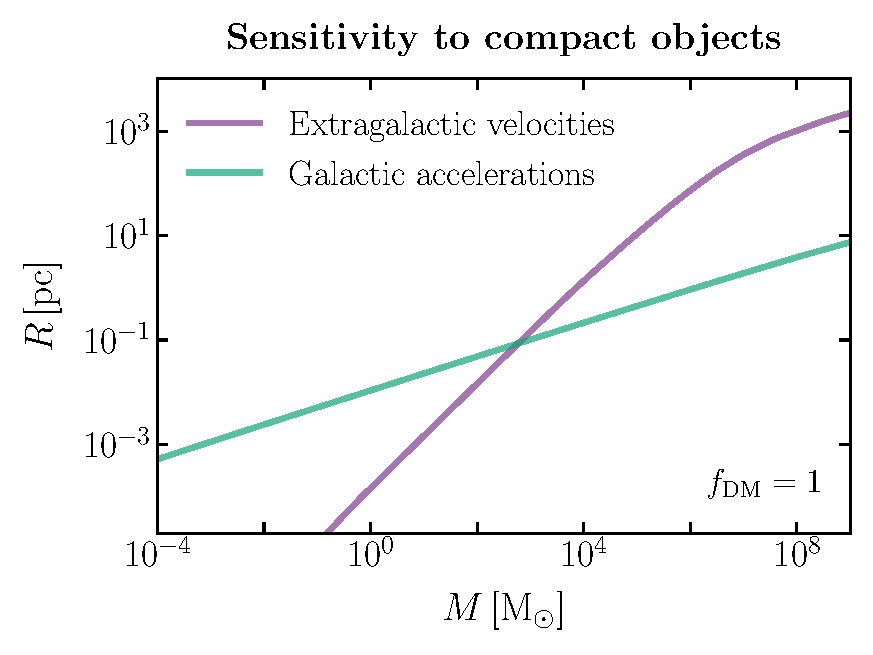
\includegraphics[width=0.45\textwidth]{plots/compact_M_vs_R}
  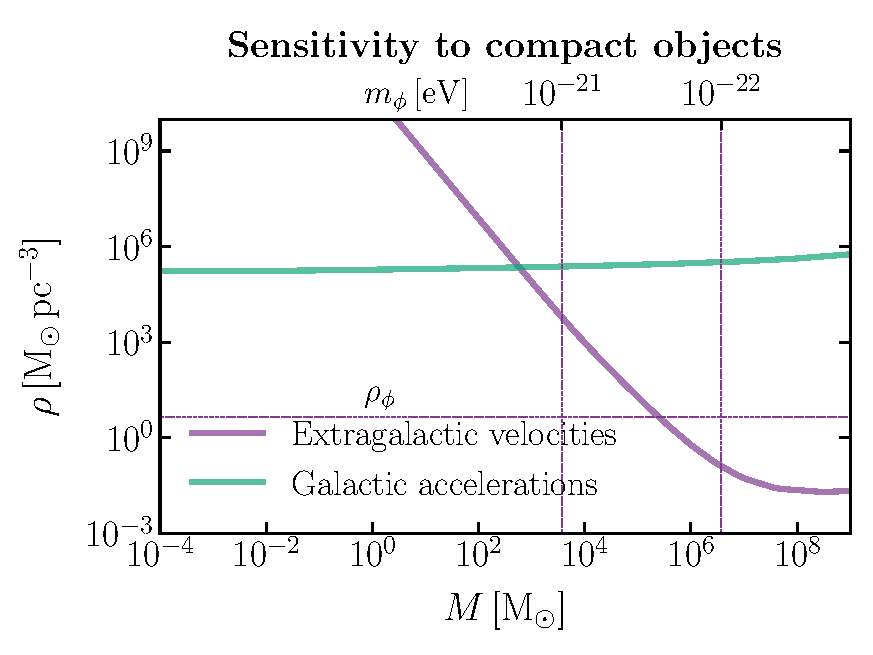
\includegraphics[width=0.48\textwidth]{plots/compact_M_vs_rho}
  \caption{(Left) Maximum subhalo size $R$ that can be constrained at 95\% confidence as a function of subhalo mass $M$, and (Right) Maximum subhalo density $\rho$ that can be constrained at 95\% confidence as a function of subhalo mass $M$, assuming dark matter fraction $f_\mathrm{DM}=1$. The dashed lines represent the density (horizontal) and masses (vertical) of unbound fluctuations in the case of scalar field dark matter with benchmark masses $m_\phi = 10^{-22}$ and $10^{-21}$\,eV.} 
  \label{fig:compact_sens}
\end{figure*}

% \begin{figure*}[htbp]
%   \centering
%   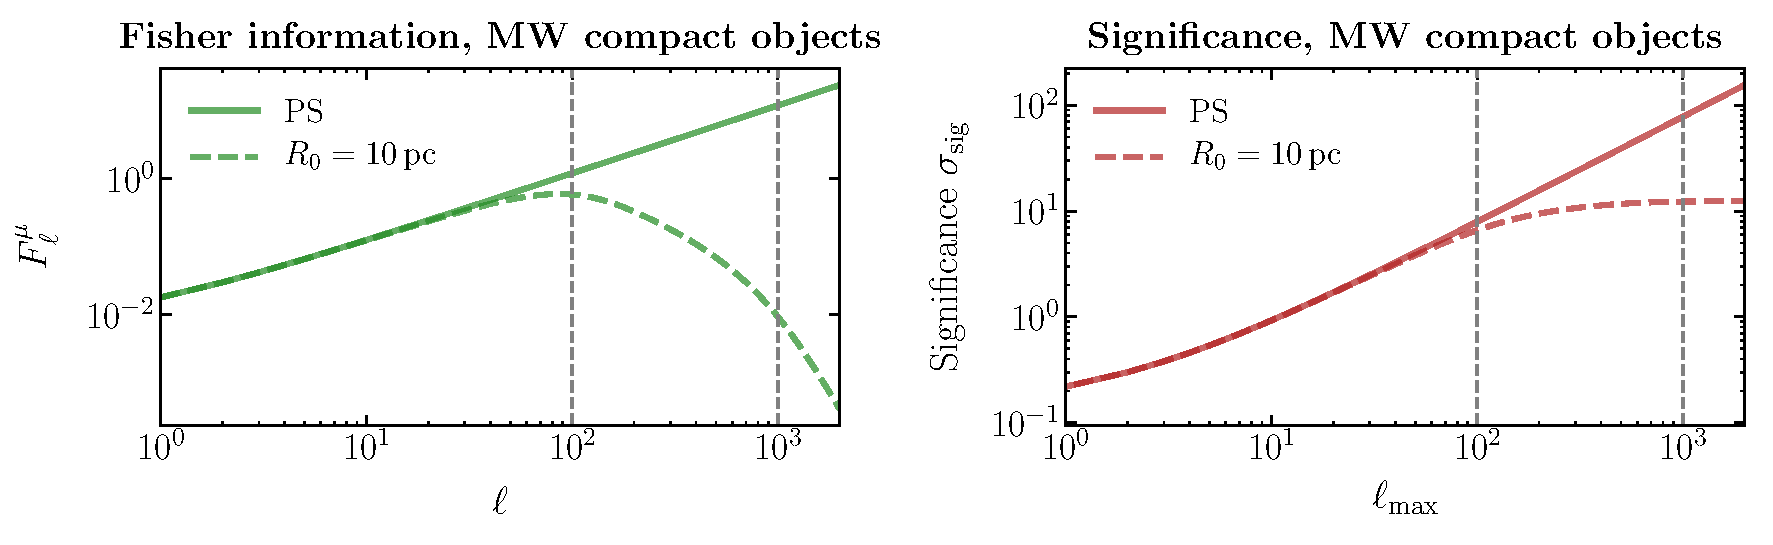
\includegraphics[width=0.9\textwidth]{plots/fisher_mu_mw}
%   \caption{Fisher information and significance for compact objects in the Milky Way, shown for point source (solid) and extended with $R_0=10\,\mathrm{pc}$.} 
%   \label{fig:fisher_sig_mw}
% \end{figure*}

\subsection{Cold dark matter}
\label{sec:cdmpop}

The cold dark matter (CDM) paradigm has been extremely successful in explaining the distribution of structure at large scales, and predicts a broad spectrum of subhalo masses on sub-Galactic scales. Figure~\ref{fig:compact_sens} (Right) hints at the potential sensitivity of using induced, correlated proper motions to infer a population of CDM subhalos, since these would be expected to be extended (at the $\sim$kpc scale for masses of $10^8\,\mathrm{M}_\odot$) and potentially within reach of future astrometric surveys. We start by describing our CDM-inspired fiducial model.

\begin{itemize}
\item \emph{Subhalo mass function:} Numerical simulations show that the (sub)halo mass function $dN/dM$ in $\Lambda$CDM can be well-described as nearly scale-invariant by a power-law distribution of the form $dN/dM\propto M^{-\alpha}$ with $\alpha\approx1.9$--$2$~\cite{Moline:2016pbm} over a large range of masses. We set $\alpha=1.9$ in our fiducial configuration, consistent with simulations of Milky Way-sized halos~\cite{Madau:2008fr,Springel:2008cc}. We also investigate a steeper mass function with $\alpha=2$, leading to a larger relative abundance of lower-mass subhalos.

To calibrate the amplitude of the mass function, we require $N_\mathrm{calib}=150$ subhalos in expectation between $10^8$--$10^{10}$\,M$_\odot$~\cite{Hutten:2016jko}, consistent with results from recent hydrodynamical simulations~\cite{Mollitor:2014ara,Sawala:2015cdf}. The threshold minimum and maximum allowed subhalo masses are fixed at $10^{-6}$\,M$_\odot$ and $0.05\,M_\mathrm{MW}$~\cite{Hiroshima:2018kfv} respectively. This configuration leads to $\sim 19\%$ of the total Milky Way mass bound in substructure. We also investigate a more subhalo-rich configuration, setting $N_\mathrm{calib}=300$, consistent with the results of DM-only simulations~\cite{Springel:2008cc}.

\item \emph{Spatial distribution of subhalos:}  While the unevolved (infall) subhalo spatial distribution is expected to follow the smooth Milky Way halo profile, tidal disruption due to the gradient of the Galactic potential towards the Galactic Center is expected to deplete the fraction of mass bound in substructures there. We account for this by describing the spatial distribution of subhalos using an Einasto profile with a fit to the results of the Aquarius simulation~\cite{Springel:2008cc,Hutten:2016jko}, 

\begin{equation}
\rho(r) = \exp\left[-\frac{2}{\alpha_\mathrm{E}}\left(\left(\frac{r}{r_\mathrm{E}}\right)^{\alpha_\mathrm{E}} - 1\right)\right]
\end{equation}
with $r_\mathrm{E}=199$\,kpc and $\alpha_\mathrm{E}=0.678$.

There are indications that some portion of the subhalo tidal disruption effects observed in simulations could be numerical in origin~\cite{vandenBosch:2017ynq,vandenBosch:2018tyt}. We account for this possibility by by investigating the scenario where the evolved distribution of subhalo follows the smooth Galactic dark matter profile.

\item \emph{Subhalo profile:} We model the subhalos with an NFW profile, using the Galactic Center distance-dependent concentration-mass relation from Ref.~\cite{Moline:2016pbm} in our fidicual set-up which takes into account the larger concentration of subhalos as compared to field halos closer to the Galactic center due to tidal distruption effects. We explore the dependence on the concentration-mass parameterization by using the alternate model from Ref.~\cite{Correa:2015dva}.

\end{itemize}

The total poloidal induced proper motion power spectrum signal expected for the fiducial configuration, as well as the alternate modeled scenarios, is shown in Fig.~\ref{fig:lcdm_theory}. The fiducial CDM model is shown in purple. Not accounting for tidal disruption~\cite{vandenBosch:2017ynq,vandenBosch:2018tyt} preferentially bringing subhalos closer to the Galactic Center and boosts the signal by about an order of magnitude at all scales (green line). A steeper subhalo mass function with $\alpha=-2$ (blue line) results in a larger number of low-mass subhalos, slightly boosting the signal on small scales and depressing it on larger scales. 

\begin{figure}[htbp]
  \centering
  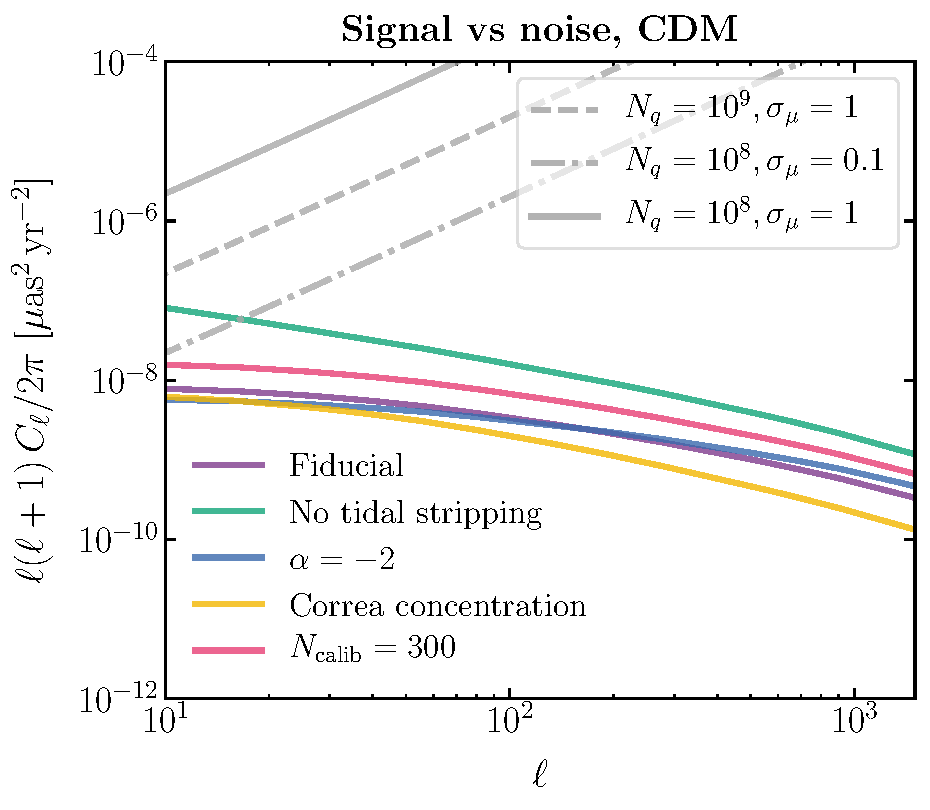
\includegraphics[width=0.45\textwidth]{plots/LCDMTheoryNoise}
  \caption{The total signal power spectrum expected for the fiducial CDM-inspired subhalo configuration described in Sec.~\ref{sec:cdmpop} (blue line). Noise spectra for a few representative cases, parameterized by the proper motion variance $\sigma_\mu$ and number of observed quasars $N_q$ are shown as the dot-dashed, dashed and solid grey lines for increasingly optimistic observation scenarios.} 
  \label{fig:lcdm_theory}
\end{figure}

It is instructive to ask which regions of the subhalo mass and spatial distribution phase space contribute to the total power spectrum signal. The differential spectra $d\ln C_\ell/d\ln M_{200}$ and $d\ln C_\ell/d\ln R$ are shown in Fig.~\ref{fig:pspec_differential} for multipoles $\ell=10, 30, 100$. It can be seen that larger scales receive preferential contribution from subhalos that are massive and/or closer in Galactocentric radius, as intuitively expected. It can also been seen that, at accessible scales, the dominant contribution comes from the population of subhalos at intermediate Galactocentric radii ($R\sim50$--$150$\,kpc). This underscores the fact that the lensing signal is derived in aggregate from a population of subhalos, and the power spectrum measurement is probing the substructure population in the bulk Galactic halo.


\begin{figure*}[!htbp]
  \centering
  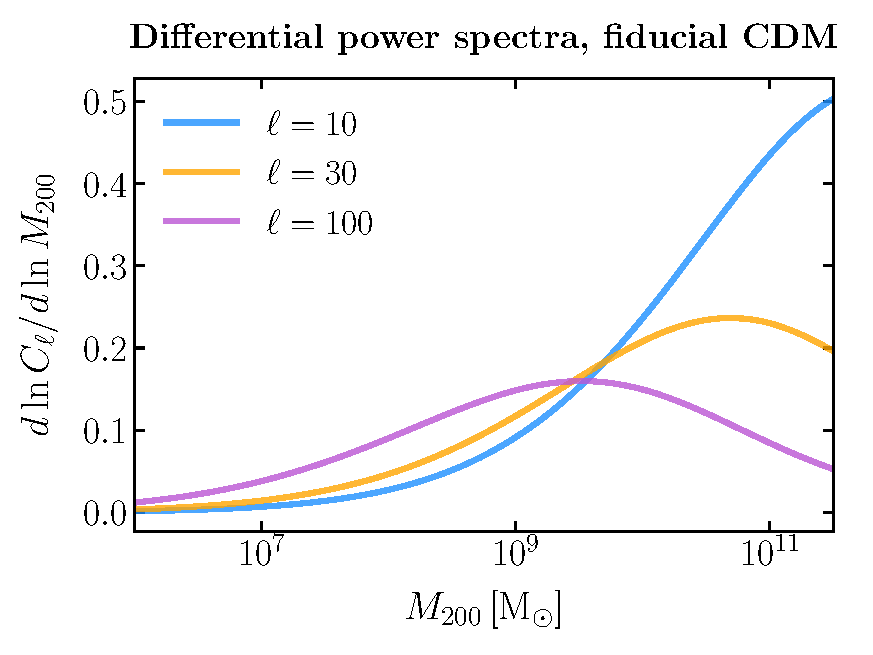
\includegraphics[width=0.45\textwidth]{plots/dlnCldlnM200}
  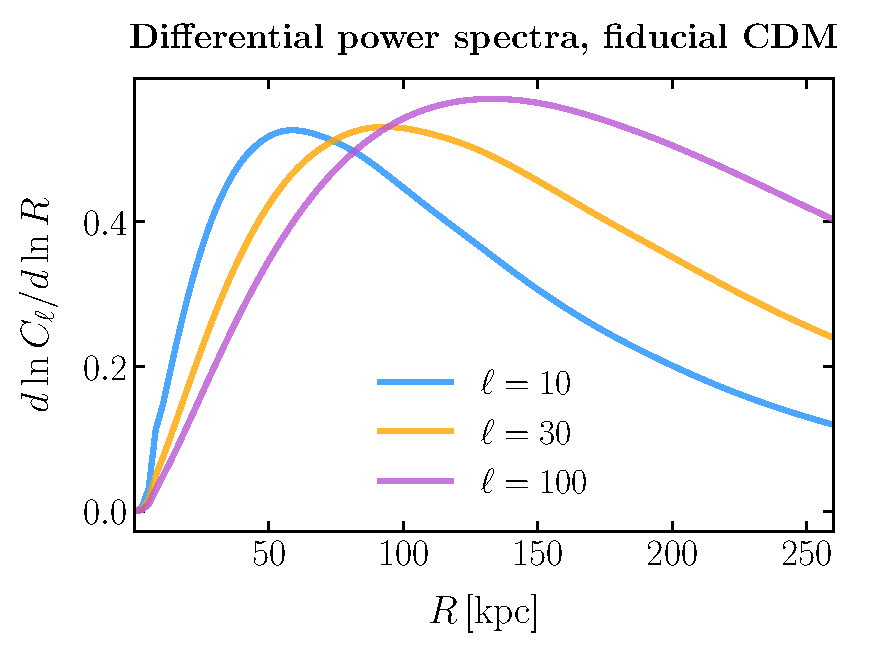
\includegraphics[width=0.45\textwidth]{plots/dlnCldlnR}
  \caption{Mass (left) and Galactocentric distance (right) dependence of the total proper motion power spectrum at multipoles $\ell=10$ (blue), $\ell=30$ (yellow) and $\ell=1000$ (purple).} \label{fig:pspec_differential}
\end{figure*}

Using the procedure outlined in App.~\ref{sec:fisher}, we may finally obtain the sensitivity of a given set of observations to a given signal configuration. Figure~\ref{fig:lcdm_disc} shows the discovery significance for the fiducial CDM configuration (left) and the optimistic configuration without tidal stripping (right), using quasar velocity power spectra, for different values of the proper motion noise $\sigma_\mu$ and number of observed quasars $N_q$. We see that the optimistic scenario may be within reach of the next generation of interferometric telescopes, assuming noise levels $\sigma_\mu\approx 1\,\mu$as\,yr$^{-1}$ and $N_q\approx10^8$. Prospects assuming the fiducial scenario accounting for tidal disruption are less promising, and will require methods beyond those presented here (see Sec.~\ref{sec:conclusions}), or astrometric precision beyond that expected with next generation surveys.

\begin{figure*}[htbp]
  \centering
  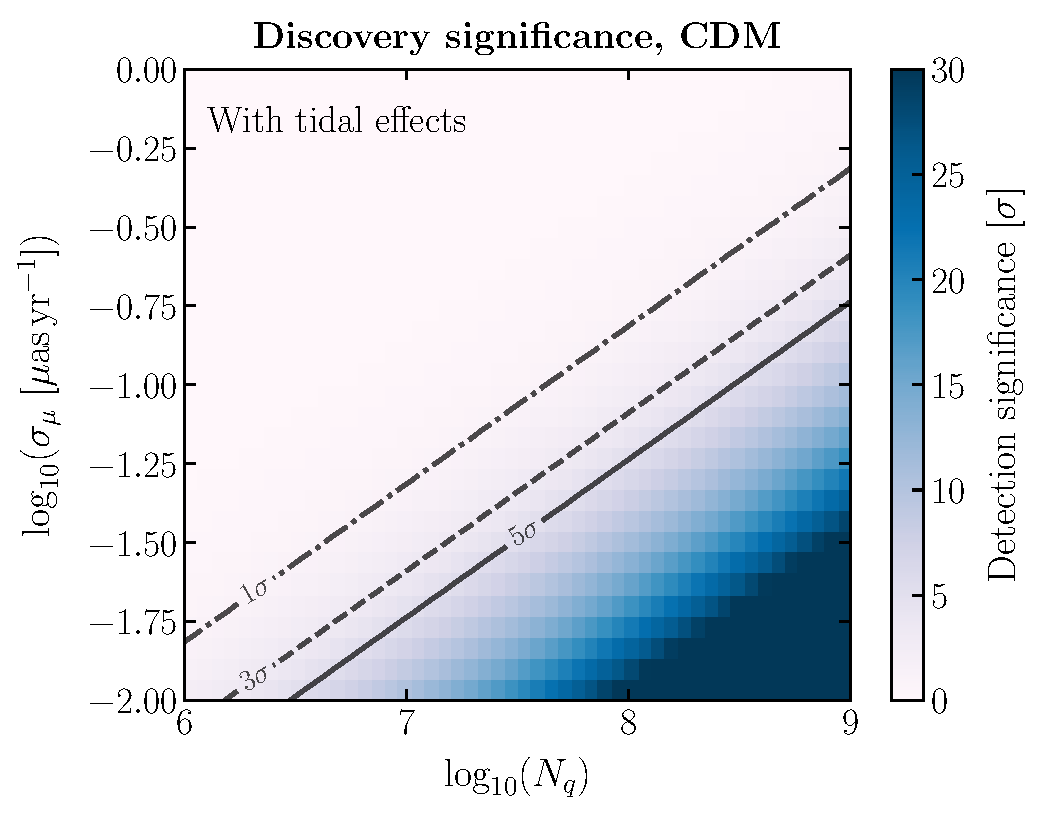
\includegraphics[width=0.45\textwidth]{plots/LCDM_disc}
  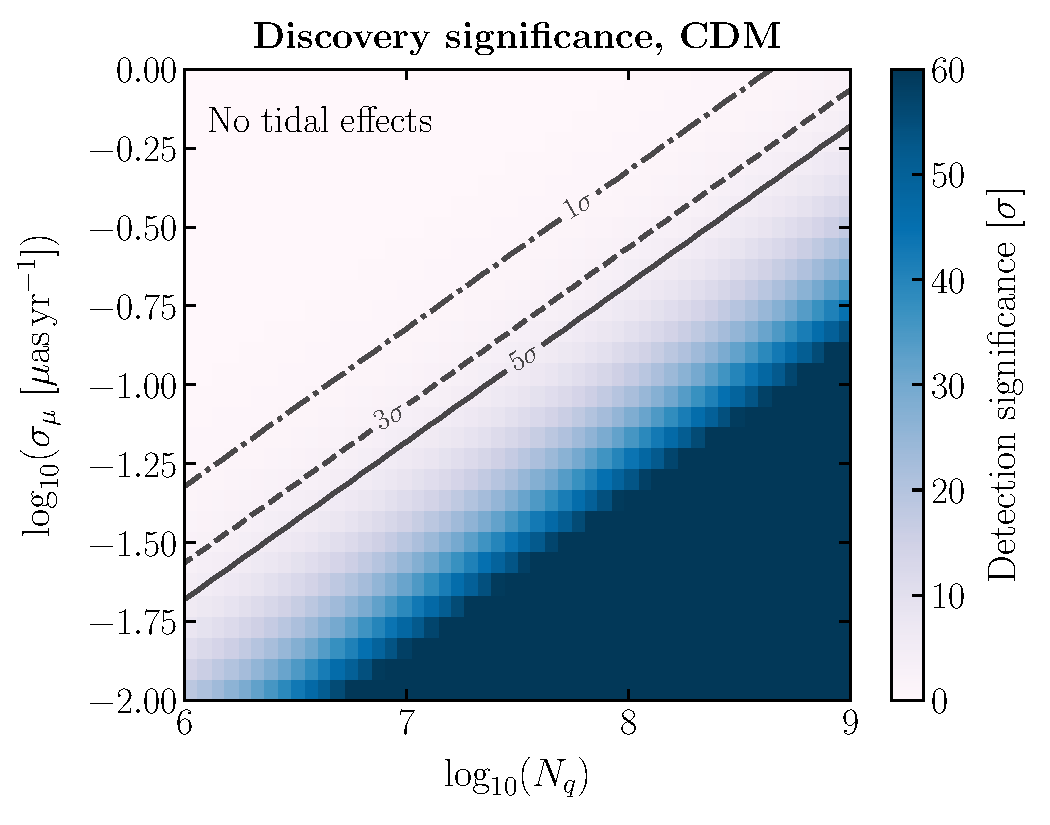
\includegraphics[width=0.45\textwidth]{plots/LCDM_disc_notidal}
  \caption{Discovery significance of the fiducial CDM-inspired scenario using quasar velocity power spectra, shows as a heatmap for different values of the proper motion noise $\sigma_\mu$ and number of observed quasars $N_q$.} \label{fig:lcdm_disc}
\end{figure*}

% It is instructive to consider the sensitivity of the forecasts to the minimum and maximum angular scales considered. Fig.~\ref{fig:lcdm_lminlmax} shows the improvement expected over the baseline case with $l_\mathrm{min} = 10$, $l_\mathrm{max} = 300$ for different values of $l_\mathrm{min}$ and $l_\mathrm{max}$. It can be seen that, for the fiducial setup and noise configuration, the sensitivity mainly comes from larger scales $\ell\sim10$--$30$.

% \begin{figure}[htbp]
%   \centering
%   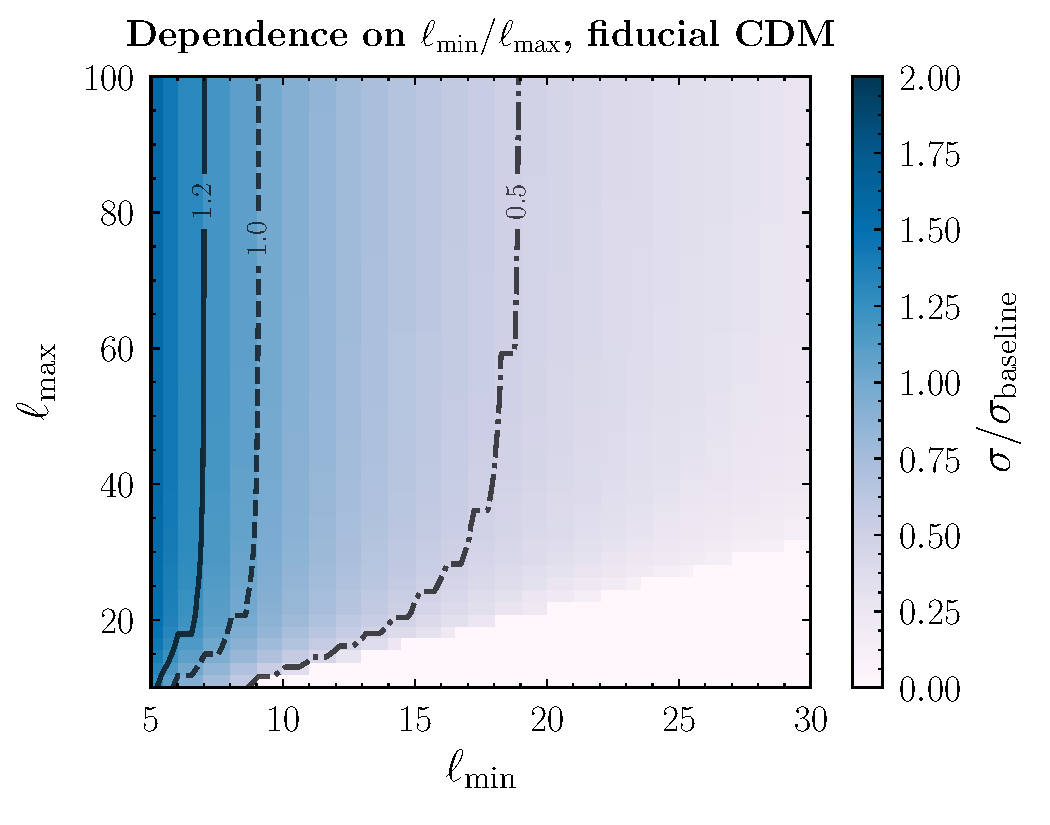
\includegraphics[width=0.45\textwidth]{plots/LCDM_lminmax}
%   \caption{Improvement in detection significance with respect to the baseline configuration $l_\mathrm{min} = 10$, $l_\mathrm{max} = 300$.} 
%   \label{fig:lcdm_lminlmax}
% \end{figure}

% \subsubsection*{Simulations}

% It is useful to verify the formalism presented above on simulated data. We simulate subhalo realizations consistent with our fiducial CDM model, for computational tractability going down to a minimum subhalo mass of $M_{200} = 10^{6.5}$\,M$_\sun$ and inducing deflections on quasars up to $20^\circ$ from the lens position. The toroidal velocity power spectrum measured over 200 realizations is shown in Fig.~\ref{fig:theoryvssim}, the pink band specifying the middle 50\% containment. The theoretically calculated power spectrum for this configuration is shown in blue. It can be seen that the set of approximations used for the analytic calculation start breaking down at larger scales $\ell\lesssim30$, but the theoretical prediction remains well within middle 50\% containment in the relevant multipole range considered. 


% \begin{figure}[!htbp]
%   \centering
%   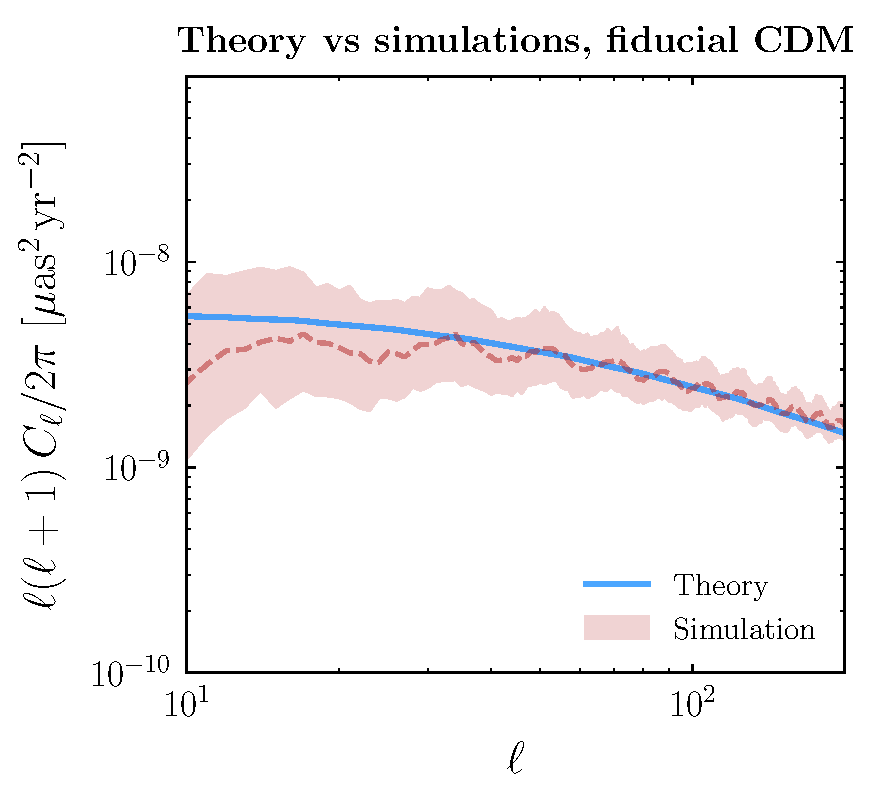
\includegraphics[width=0.44\textwidth]{plots/TheoryvsSim}
%   \caption{Theoretical velocity power spectrum calculated with Eq.~\ref{eqn:popcell} (blue) compared with that measured from simulations (red), shown as the median and middle 50\% over 200 realizations. }
%   \label{fig:theoryvssim}
% \end{figure}

\subsection{Scalar dark matter}

In this section, we compute the power spectrum of the velocity and acceleration distortion in a halo made up of real scalar dark matter. The contribution to the power calculated below is irreducible because it originates from the unavoidable density fluctuations of a free scalar field at the scale of the typical de Broglie wavelength in a thermal ensemble. Assuming the velocity spectrum and density distribution of the halo is known, the velocity and acceleration power has only one free parameter --- the scalar field's mass $m$. 
\begin{align} 
\left\langle a_{\vect{k}}^\dagger a_{\vect{q}} \right\rangle = n_0 f(\vect{k}) \deltabarthree(\vect{k}-\vect{q}) \label{eq:scalarensemble}
\end{align}
The total particle number density is $n_0$, and $f(\vect{k})$ is defined as the momentum distribution with $\int \ddbar^3 k \, f(\vect{k}) = 1$.
All other contractions with the external state, e.g.~those of the form $\langle a a \rangle$ and $\langle a^\dagger a^\dagger\rangle$ are assumed to be zero, as we expect virialization to scramble all phase information. We will also effectively take all commutators $[a_{\vect{k}}^\dagger, a_{\vect{q}}] = 0$, since it can be shown that terms involving commutators are suppressed by inverse powers of the occupation number $n_0 / \sigma_k^3\gg 1$ where $\sigma_k$ is a typical momentum, i.e.~we are doing a classical expansion. Expressing the field as a superposition of momentum modes,
\begin{align}
\phi(x) = \int \frac{\ddbar^3 k}{\sqrt{2k^0}} \left(a_{\vect{k}} e^{-i k \cdot x} + a_{\vect{k}}^\dagger e^{+i k\cdot x}\right),
\end{align}
with $k^0 \equiv \sqrt{m^2 + \vect{k}^2}$, we can compute expectation values such as $\langle \phi \rangle = 0$ and that of the density $\rho = [\dot{\phi}^2 + (\nabla \phi)^2 + m^2 \phi^2] /2$:
\begin{align}
\langle \rho \rangle =  n_0 \int \ddbar^3 k\, f(\vect{k}) k^0 \simeq n_0 m \equiv \rho_0.
\end{align}
The approximate equality holds for a nonrelativistic momentum distribution, the case of interest. 

The aforementioned density fluctuations give rise to a nontrivial density correlation function
%\begin{widetext}
\begin{align}
&\langle \rho(x) \rho(x') \rangle = \langle \rho \rangle^2 + \frac{n_0^2}{4} \int \frac{\ddbar^3 k_1}{k^0_1} \, \frac{\ddbar^3 k_2}{k^0_2} \,  f(\vect{k}_1) f(\vect{k}_2) \label{eq:rhocorr}
 \\
&\Bigg\lbrace \left[m^2 -  k^0_1 k^0_2 - \vect{k}_1 \cdot \vect{k}_2 \right]^2\cos\left[(k_1 + k_2)\cdot (x-x')\right] \nonumber\\
&\phantom{\Bigg \lbrace} + \left[m^2 +  k^0_1 k^0_2 + \vect{k}_1 \cdot \vect{k}_2 \right]^2 \cos\left[(k_1 - k_2)\cdot (x-x')\right]  \Bigg\rbrace \nonumber
\end{align}
%\end{widetext}
from which it can be read off that the fractional variance of $\rho$, namely ($\langle \rho^2 \rangle - \langle \rho \rangle^2)/\langle \rho\rangle^2$, is order unity. There are thus irreducible, \emph{unbound} $\mathcal{O}(1)$ density fluctuations in a virialized scalar dark matter halo, regardless of cosmological history and the \emph{bound} substructure of the halo, of which there is generally less with ultralight scalar dark matter than with CDM~\cite{}.\footnote{Note that large-field scalar dark matter models have \emph{more} bound substructure.}
In what follows, we will take
\begin{align}
f(\vect{k}) = \frac{(2\pi)^{3/2}}{\sigma_k^3} \exp\left\lbrace-\frac{(\vect{k}-\vect{k}_\odot)^2}{2\sigma_k^2} \right\rbrace \label{eq:fmom}
\end{align}
where the momentum dispersion is $\sigma_k \equiv m \sigma_v$ with $\sigma_v \approx 166\,\mathrm{km \, s^{-1}}$ and the average momentum in the Sun's rest frame is $\vect{k}_\odot \equiv m \vect{v}_\odot$.
The typical mass $M_0$ and radius $R_0$ of these overdensities is thus of order:
\begin{align}
M_0 &= C \rho_0 \left(\frac{\pi}{\sigma_k}\right)^3 \approx 5 \times 10^5 M_\odot\,C m_{22}^{-3}\label{eq:scalarM0}\\
R_0 &= \frac{1}{2\sigma_k} \approx 58\,\mathrm{pc}\, m_{22}^{-1} \label{eq:scalarR0}
\end{align}
with $m_{22} \equiv m / 10^{-22}\,\mathrm{eV}$. Since $\phi$ is a Gaussian random field, not all overdensities contain the same mass, but as we will see below, the constant $C$ can be made more precise in the context of the lensing-induced power spectra.

We will now compute to what degree these density fluctuations cause distortions in proper motions and accelerations of luminous sources. Defining the Fourier transform of the observable $\mathcal{O}$ to be $\tilde{\mathcal{O}}(\vect{k}) = \int \ddbar^3k \, e^{-i \vect{k} \cdot \vect{x} } \mathcal{O}(\vect{x}) $ and its power spectrum $\langle \tilde{\mathcal{O}}(\vect{k}) \tilde{\mathcal{O}}(\vect{k}')^*  \rangle \equiv P_{\mathcal{O}}(\vect{k}) \deltabarthree(\vect{k}-\vect{k}')$, we can compute from Eq.~\ref{eq:rhocorr} the power spectrum of $\dot{\rho}$:
%\begin{align}
%P_{\rho}(\vect{k}) \simeq \frac{\rho_0^2}{2} \int \ddbar^3 q\, f(\vect{q}) \left[f(\vect{k}-\vect{q}) + f(-\vect{k}-\vect{q}) \right]
%\end{align}
\begin{align}
P_{\dot{\rho}}(\vect{k}) &\simeq \frac{\rho_0^2}{8m^2} \int \ddbar^3 q\, f(\vect{q}) \big[(\vect{k}^2 - 2\vect{k}\cdot \vect{q})^2 f(\vect{k}-\vect{q})  \\
 &\hspace{10em}+(\vect{k}^2 + 2\vect{k}\cdot \vect{q})^2 f(-\vect{k}-\vect{q}) \big] \nonumber\\
 &= \frac{\pi^{3/2}}{4} \frac{\rho_0^2}{m^2 \sigma_k} (\vect{k}^2 + 8 \vect{k}_{\odot}^2) \left[e^{-\frac{(\vect{k}+2\vect{k}_\odot)^2}{4\sigma_k^2}}+e^{-\frac{(\vect{k}-2\vect{k}_\odot)^2}{4\sigma_k^2}} \right]\nonumber.
\end{align}
In the second line, we evaluated the integral with the momentum distribution of Eq.~\ref{eq:fmom}. The above power spectrum is computed from the equal-time correlation function $\langle \dot{\rho}(t,\vect{x}) \dot{\rho}(t,\vect{x}') \rangle$ keeping only the ``slow'' term in the third line of Eq.~\ref{eq:rhocorr}, and dropping the ``fast'' term of the second line.\footnote{The fast term is not only suppressed in magnitude but averages down out severely when integrated over two lines of sight. It is justified to compute the power on the equal-time correlation function of the slow term because the coherence time $t_\mathrm{coh} \sim m/\sigma_k^2$ is much longer than the light crossing time of a de Broglie fluctuation $t_\mathrm{cross} \sim 1/\sigma_k$.} Along the same lines, we have the $\ddot{\rho}$ spectrum:
\begin{align}
P_{\ddot{\rho}}(\vect{k}) &\simeq \frac{\rho_0^2}{32m^4} \int \ddbar^3 q\, f(\vect{q}) \big[(\vect{k}^2 - 2\vect{k}\cdot \vect{q})^2 f(\vect{k}-\vect{q}) \\
 &\hspace{10em}+(\vect{k}^2 + 2\vect{k}\cdot \vect{q})^2 f(-\vect{k}-\vect{q}) \big] \nonumber\\
 &= \frac{3\pi^{3/2}}{8} \frac{\rho_0^2\sigma_k}{m^4} (\vect{k}^2 + 8 \vect{k}_{\odot}^2)^2 \left[e^{-\frac{(\vect{k}+2\vect{k}_\odot)^2}{4\sigma_k^2}}+e^{-\frac{(\vect{k}-2\vect{k}_\odot)^2}{4\sigma_k^2}} \right]\nonumber.
\end{align}
These spatio-temporal density fluctuations will give rise to corresponding fluctuations in the gravitational potential $\Phi$ through the gravitational Poisson equation: $\nabla^2 \Phi = 4 \pi G_N \rho$. The power spectra of the gravitational potential fluctuations can thus be written as $P_{\dot{\Phi}}(\vect{k}) = (4\pi G_N)^2 P_{\dot{\rho}}(\vect{k})/\vect{k}^4$ and likewise for higher time derivatives. The reduced lensing deflection potential $\psi$ of Eq.~\ref{eq:deflectionpotential} is a line-of-sight integral of the gravitational potential, $\psi(\vect{\theta}) \equiv 2 \int_0^{z_s} \dd z \, \Phi(\vect{x}) (z_s - z)/(z_s z)$, where it is now understood that $\vect{x} = \lbrace z \vect{\theta},z\rbrace$, and $z_s$ is the source distance. Finally, we can write the harmonic coefficients of Eq.~\ref{eq:harmdecomposition} as $\mu_{\ell m}^{(1)} = - \sqrt{\ell(\ell+1)} \int \dd^2\theta\, \dot{\psi}(\vect{\theta}) Y_{\ell m}^*(\vect{\theta})$ after integrating by parts, and analogously for $\alpha_{\ell m}^{(1)}$ and $\ddot{\psi}$.

We are now in a position to calculate the angular power spectra of the proper motion and acceleration, after having collected all the necessary ingredients above:
\begin{align}
\big \langle \big|\mu_{\ell m}^{(1)}\big|^2\big\rangle &= 4 \ell(\ell+1)\int_0^{z_s} \dd z  \int_0^{z_s} \dd z'\, \frac{z_s -z}{z_s z} \frac{z_s - z'}{z_s z'} \\
&\int \dd^2 \theta \, \dd^2 \theta' \,  Y_{\ell m}^*(\vect{\theta}) Y_{\ell m}(\vect{\theta}') \int \ddbar^3 q\, P_{\dot{\Phi}}(\vect{q}) e^{i\vect{q}\cdot (\vect{x}-\vect{x}')}\nonumber,
\end{align}
and likewise for $ \langle |\alpha_{\ell m}^{(1)}|^2\rangle$ but with $P_{\ddot{\Phi}}(\vect{q})$. If we integrate the fluctuations over a sphere with constant density $\rho_0$, dispersion $\sigma_k$, and radius $D$, we take $z_s \to \infty$ and $\vect{k}_\odot = 0$, and approximate $\int_0^D \dd z \, j_\ell (q z) / z \simeq \Theta(q - \ell / D) \sqrt{\pi/2\ell^3}$, we can evaluate all integrals and find:
\begin{align}
\big \langle \big|\mu_{\ell m}^{(1)}\big|^2\big\rangle &= \underbrace{32\pi^4 \frac{G_N^2 \rho_0^2}{m^2}}_{1.3 \times 10^{-8} \frac{\mu\mathrm{as}^2}{\mathrm{y}^{2}} m_{22}^{-2}} \frac{\mathrm{erfc}(\frac{\ell}{2\sigma_k D})}{\ell} 
\\
%&\approx 1.3  \times 10^{-8} \mu\mathrm{as}^2\, \mathrm{y}^{-2} \left[ \frac{10^{-22}\,\mathrm{eV}}{m}\right]^2 \frac{\mathrm{erfc}(\frac{\ell}{2\sigma_k D})}{\ell}  \nonumber
\big \langle \big|\alpha_{\ell m}^{(1)}\big|^2\big\rangle &= \underbrace{96\pi^4 G_N^2 \rho_0^2 \sigma_v^4}_{8.4 \times 10^{-20} \frac{\mu\mathrm{as}^2}{\mathrm{y}^{4}}}\frac{\mathrm{erfc}(\frac{\ell}{2\sigma_k D})+\frac{\ell}{\sqrt{\pi}\sigma_k D} e^{-\frac{\ell^2}{4\sigma_k^2 D^2}}}{\ell} \nonumber
%&\approx 8.4 \times 10^{-20} \mu\mathrm{as}^2\, \mathrm{y}^{-4} \frac{\mathrm{erfc}(\frac{\ell}{2\sigma_k D})+\frac{\ell}{\sqrt{\pi}\sigma_k D} e^{-\ell^2/4\sigma_k^2 D^2}}{\ell}   \nonumber
\end{align}
It can be shown that one gets exactly the same angular power spectrum (with the same assumptions on $\rho_0, \sigma_k$, $D$, $z_s$, and $\vect{v}_\odot$) for an ensemble of Gaussian lenses (Eq.~\ref{eq:Gaussianrho}) with uniform number density $\rho_0/M_0$, and mass $M_0$ and radius $R_0$ from Eqs.~\ref{eq:scalarM0} and \ref{eq:scalarR0}, assuming $C = 4/3\pi^{3/2}$ for $\big \langle \big|\mu_{\ell m}^{(1)}\big|^2\big\rangle$ and $C = 32/15\pi^{3/2}$ for $\big \langle \big|\alpha_{\ell m}^{(1)}\big|^2\big\rangle$. This means we can plot the sensitivity to scalar dark matter in the parameter space for compact objects explored in Sec.~\ref{sec:compact}. This is shown in the right panel of Fig.~\ref{fig:compact_sens} as the dotted horizontal and vertical lines denoting the densities and masses respectively of scalar field dark matter particles for benchmark points $m_\phi = 10^{-22}$ and $10^{-21}$\,eV.

% To calculate the velocity power spectrum, we need the correlation function of the first time derivative of the gravitational potential:
% \begin{align}
% \left\langle \dot{\Phi}(\vect{y}) \dot{\Phi}(\vect{y}') \right\rangle &= (4\pi G_N)^2 \int \ddbar^3 k \, \ddbar^3 k' \, \frac{e^{i(\vect{k}\cdot \vect{y} + \vect{k}' \cdot \vect{y}')}}{\vect{k}^2 \vect{k}^{\prime 2}}\\
% &\phantom{=} \hspace{0em} \times \int \dd^3 x \, \dd^3 x' \, e^{-i(\vect{k}\cdot \vect{x} + \vect{k}' \cdot \vect{x}')} \left \langle \dot{\rho}(\vect{x}) \dot{\rho}(\vect{x}') \right \rangle \nonumber\\
% &\simeq \frac{\sqrt{\pi}}{8} (4 \pi G_N)^2 n_0^2 \frac{\mathrm{erf}\left(\sigma_k |\vect{y}-\vect{y}'|\right)}{\sigma_k |\vect{y}-\vect{y}'|}
% \end{align}
% Likewise, for the acceleration power spectrum, we need the equivalent second-time-derivative correlator:
% \begin{align}
% \left\langle \ddot{\Phi}(\vect{y}) \ddot{\Phi}(\vect{y}') \right\rangle = \dots
% \end{align}

% Real-space velocity correlation function:
% \begin{align}
% &\left\langle \vect{\mu}(\vect{\theta}) \cdot \vect{\mu}(\vect{\theta}') \right\rangle \\
% &\hspace{0em} = 4 \int_0^D \frac{\dd z}{z} \int_0^D \frac{\dd z'}{z'} \nabla_\theta \cdot \nabla_{\theta'} \left\langle \dot{\Phi}(z\vect{\theta},z) \dot{\Phi}(z'\vect{\theta}',z') \right\rangle \nonumber \\
% &\hspace{0em} \simeq \frac{\sqrt{\pi}}{2} (4\pi G_N)^2 \frac{\rho_0^2 \sigma_v D}{m} F^{(\mu)}\left[ |\vect{\theta}-\vect{\theta}'|,\sigma_k D \right] \nonumber \\
% &\approx 1.0 \times 10^{-7}~\mathrm{\frac{\mu as^2}{y^2}} \left( \frac{10^{-22}~\mathrm{eV}}{m} \right)  \left(\frac{D}{10~\mathrm{kpc}}\right) \left(\frac{F^{(\mu)}}{2} \right)
% \end{align} %\left\langle \dot{\Phi}(\vect{y}) \dot{\Phi}(\vect{y}') \right\rangle
% \blue{One of the los-integrations can be done in closed (but ugly) form, but not the second one. Parametrized angular dependence into numerically computed form factor.}
% \begin{align}
% \left\langle \vect{\alpha}(\vect{\theta}) \cdot \vect{\alpha}(\vect{\theta}') \right\rangle = \dots
% \end{align}
% \begin{align}
% \sigma_k D \approx 86  \left( \frac{10^{-22}~\mathrm{eV}}{m} \right)  \left(\frac{D}{10~\mathrm{kpc}}\right) 
% \end{align}

% \begin{figure}[htbp]
%   \centering
%   \includegraphics[width=0.45\textwidth]{../figs/plt_muFform.pdf}
%   \includegraphics[width=0.45\textwidth]{../figs/plt_muGform.pdf}
%   \caption{Form factor for real-space velocity correlation function $F^{(\mu)}$ and power spectrum form factor $G^{(\mu)}$ (multiplied by $\ell^2$. Solid = positive, dashed = negative. \blue{need to get rid of numerical noise}.} 
%   \label{fig:muForm}
% \end{figure}

% ``Flat'' power spectrum with $\vect{\mu}(\vect{\ell}) = \int \dd^2 \theta\, e^{-i \vect{\ell} \cdot \vect{\theta}} \vect{\mu}(\vect{\theta})$:
% \begin{align}
% \left\langle |\vect{\mu}(\vect{\ell})|^2 \right\rangle &= \int \dd^2 \theta\, \dd^2 \theta'\, e^{-i \vect{\ell} \cdot (\vect{\theta} - \vect{\theta}')} \left\langle \vect{\mu}(\vect{\theta}) \cdot \vect{\mu}(\vect{\theta}') \right\rangle \\
% &= \Delta \Omega \, \pi^{3/2} (4\pi G_N)^2 \frac{\rho_0^2 \sigma_v D}{m} G^{(\mu)}\left[ \ell, \sigma_k D \right] \nonumber
% \end{align}
% with $G^{(\mu)}\left[ \ell, \sigma_k D \right] \equiv \int_0^\pi \dd \theta\, \theta J_0(\ell \theta) F^{(\mu)}(\theta, \sigma_k D)$. The $G^{(\mu)}$ form factor (multiplied by $\ell^2$) is plotted in Fig.~\ref{fig:muForm}.
% \subsection{Precision halometry}

\subsection{Enhanced Primordial Power}

We investigate here a scenario in which the spectrum of primordial perturbations is enhanced at small scales. Compared to the standard $\Lambda$CDM scenario, this leads to an overabundance of low-mass halos which, having collapsed at earlier times, would also be significantly denser compared to the standard cosmological evolution. We model this enhancement by introducing a kink in the dimensionless power spectrum of Gaussian curvature perturbations $\Phi$ parameterized by a break $k_B$ and high-$k$ slope $n_B$,
\begin{align}
\mathcal{P}_{\Phi}(k) = \begin{cases} 
A_s \left( \frac{k}{k_*} \right)^{n_s -1} & k < k_B \\ 
A_s \left( \frac{k_B}{k_*} \right)^{n_s -1}\left( \frac{k}{k_B} \right)^{n_B -1} & k \ge k_B 
\end{cases}
\end{align}
where we take $A_s = 2.105\times10^{-9}$, $n_s=0.9665$ and $k_*\equiv0.05$~\cite{Aghanim:2018eyx}.%. Spectra kinked at small scales $\gtrsim 5\,\mathrm{Mpc}^{-1}\,h$ with $n_B \lesssim 3$ are completely unconstrained by current observations.

The dimensionless matter power spectrum at a given can be obtained through the matter transfer function $D(k,z)$ as
\begin{align}
\mathcal{P}_{\delta}(k,a) = \left|D\left(k,z\right)\right|^2 \mathcal{P}_{\Phi}(k) 
\end{align}
and we use \texttt{CLASS}~\cite{Blas:2011rf} to compute the transfer function. Given the present-day matter power spectrum, the mass variance (encoding the amplitude of fluctuations within a sphere of radius $R$) can be computed as 
\begin{align}
\sigma^2(R) = \int_{-\infty}^{\infty} \dd \ln k \, \mathcal{P}_{\Phi}(k) \left|D\left(k,z=0\right)\right|^2  \left| W(k,R) \right|^2
\end{align}
where  $W(k,R) = 3 (kR)^{-3}[\sin(kR)-kR\cos(kR)]$ is the Fourier transform of a top-hat smoothing function with smoothing scale $R\equiv (M / (4/3\pi\overline{\rho}_{m}))^{1/3}$.

With the mass variance in hand, the modified mass spectrum of subhalos in this scenarios is computed using the Tinker mass function~\cite{2008ApJ...688..709T} implemented in the \texttt{COLOSSUS}~\cite{2018ApJS..239...35D} code and given by
\begin{equation}
\frac{d n}{d M}=f(\sigma) \frac{\overline{\rho}_{m}}{M} \frac{d \ln \sigma^{-1}}{d M}
\end{equation}
where $f(\sigma)$ is parameterized as
\begin{equation}
f(\sigma)=A\left[\left(\frac{\sigma}{b}\right)^{-a}+1\right] e^{-c / \sigma^{2}}
\end{equation}
with the constants $A, a, b$ and $c$ calibrated to ($\Lambda$CDM) simulations (see Refs.~\cite{2008ApJ...688..709T,2018ApJS..239...35D} for further details). We calibrate the overall number of subhalos such that an unkinked power spectrum yields the same number of subhalos as in the $\Lambda$CDM case we have considered in Sec.~\ref{sec:cdmpop} (150 between $10^8$--$10^{10}$\,M$_\odot$~\cite{Hutten:2016jko}) with this pipeline. The left panel of Fig.~\ref{fig:kinked_specs} shows representative examples of kinked primordial power spectra, with the derived present-day matter power spectra and mass functions shown in the middle and right panels respectively.

\begin{figure*}[]
  \centering
  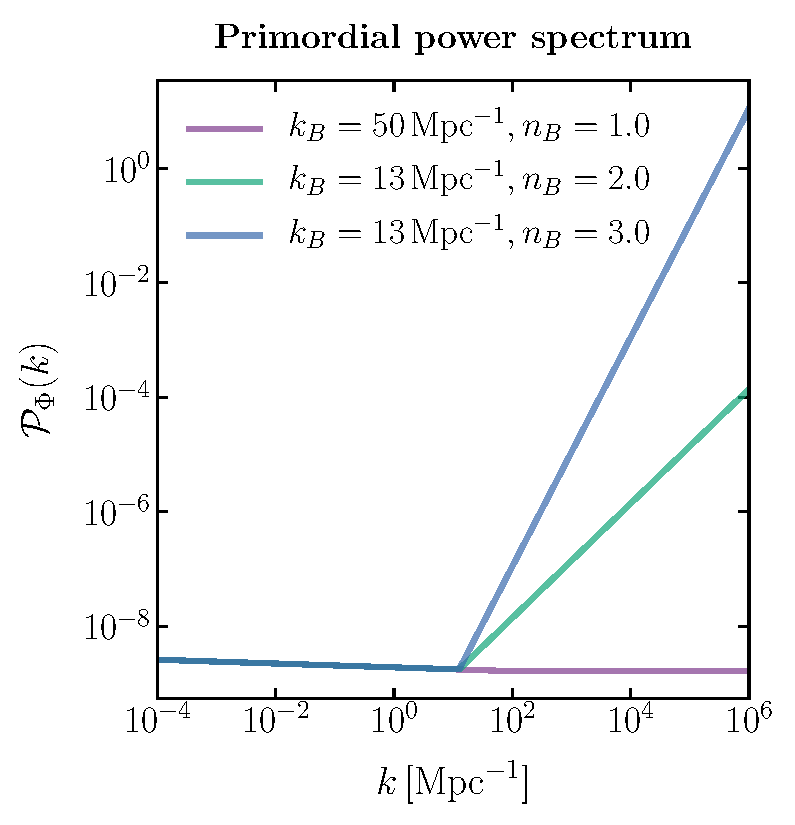
\includegraphics[width=0.32\textwidth]{plots/primordial_kinked}
  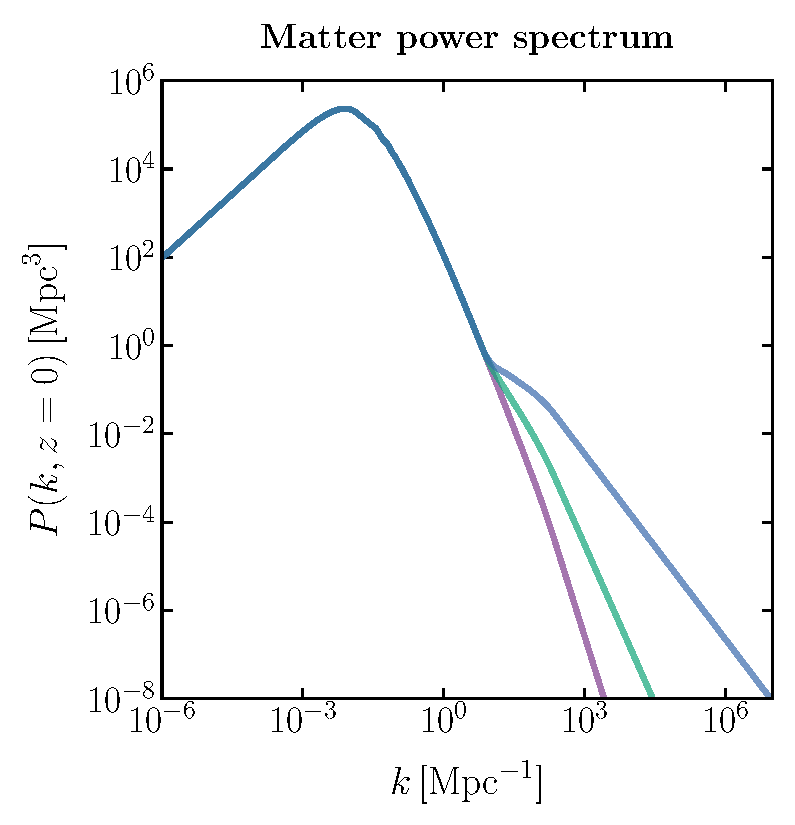
\includegraphics[width=0.32\textwidth]{plots/matterpower_kinked}
  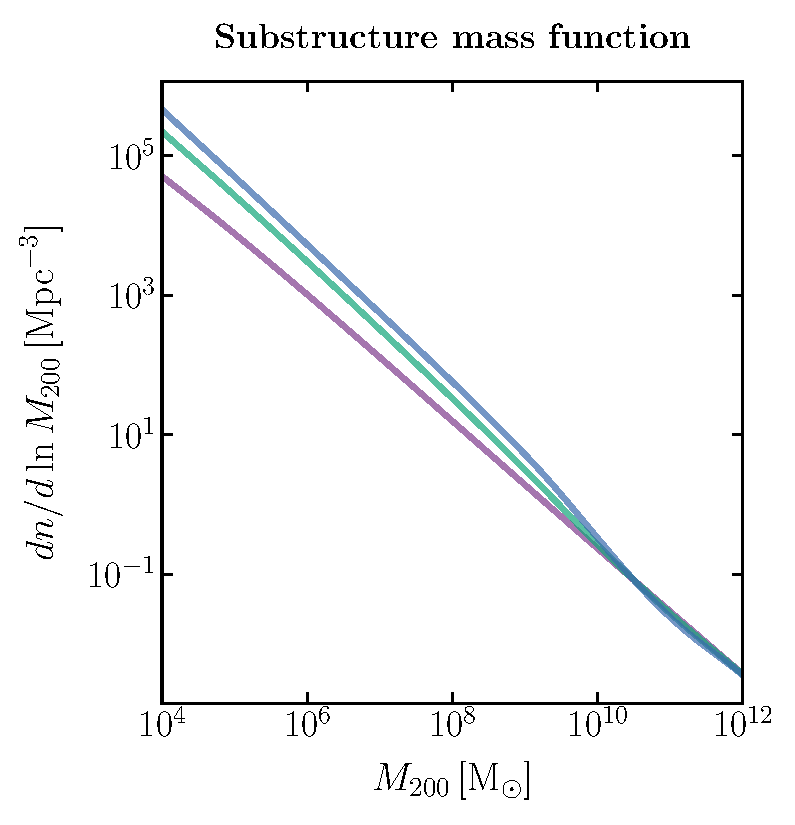
\includegraphics[width=0.32\textwidth]{plots/massfunction_kinked}
  \caption{Kinked primordial power spectra (Left) as well as derived present-day matter power spectra (Middle) and mass functions (Right) shown for the representative set of ``kink'' parameters given in the legend. A kink in the primordial power spectrum results in an overabundance of dense, low-mass substructure.}
  \label{fig:kinked_specs}
\end{figure*}

The present-day density (or equivalently, concentration) of subhalos is calculated following the procedure outlined in Ref.~\cite{Ludlow:2016ifl}. Specifically, we assume that the mean density $\langle\rho_s\rangle$ of subhalos (modeled as NFW) within the scale radius $r_s$ is proportional to the critical density of the Universe at collapse redshift $z_\mathrm{coll}$,
\begin{equation}
\frac{\langle\rho_s\rangle}{\rho_0} = C\frac{\rho_c(z_\mathrm{coll})}{\rho_0} = C\left[\frac{H(z_\mathrm{coll})}{H_0}\right]^2
\label{eq:rho_s}
\end{equation}
where $C$ is a constant to be determined. The collapse redshift corresponds to the redshift at which the current characteristic mass $M_{200}$ was contained in progenitors more massive than a fraction $f$ of this current mass.

Extended Press-Schechter theory can be invoked to relate the current characteristic mass $M_{200}$ to the scale mass~\cite{1993MNRAS.262..627L},
\begin{equation}
\frac{{M}_{s}}{{M}_{200}} \equiv \operatorname{erfc}\left(\frac{\delta_{\mathrm{sc}}\left(z_\mathrm{coll}\right)-\delta_{\mathrm{sc}}\left(z=0\right)}{\sqrt{2\left(\sigma^{2}\left(f {M}_{200}\right)-\sigma^{2}\left({M}_{200}\right)\right)}}\right)
\label{eq:M_s}
\end{equation}
where $\delta_{\mathrm{sc}}(z) \approx \delta_c / D(z)$, with $\delta_c = 1.686$, is the density threshold for collapse of a spherical top-hat perturbation and $D(z)$ the linear growth factor. The left sides of Eqs.~\ref{eq:rho_s} and \ref{eq:M_s} depend on the halos profile through the concentration $c_{200} \equiv r_{200}/r_s$. Given a present-day characteristic mass $M_{200}$, they can be simultaneously and iteratively solved to yield consistent solutions for the concentration $c_{200}$ and collapse redshift $z_\mathrm{coll}$. The constant $C$ is calibrated to yield concentrations for cluster-mass ($M_{200}\sim10^{13}\,\mathrm{M}_\odot$) halos consistent with observations for $f = 0.01$~\cite{Ludlow:2016ifl}. We choose to go down to a minimum subhalo mass of $10\,\mathrm M_\odot$ in our expository scenario to avoid extrapolating the derived concentration-mass relations and mass functions to smaller values.

95\% confidence interval sensitivity forecasts on scenarios with a kinked power spectrum are shown in Fig.~\ref{fig:kink_ps}. Shown are sensitivities achievable using quasar proper motion measurements with SKA, as well as observations of Galactic stellar proper motion accelerations by WFIRST and (end-of-mission) \Gaia. Currently unconstrained parameter space can already be probed using near-future \Gaia~astrometry.

We caution that our treatment is simplistic in several ways; it is anchored to CDM simulations at higher masses, while necessitating extrapolation of the modified power spectrum down to small scales and of the subhalo mass function and concentration-mass relation down to small subhalo masses. Although a more accurate treatment would necessarily involve \emph{N}-body simulations consistent with the modified power spectra, our semi-analytic prescription captures the essential physics while making the point that enhanced primordial fluctuations at small scales can be effectively probed with near-future astrometric observations, including the end of mission of \Gaia.


\begin{figure}[!htbp]
  \centering
  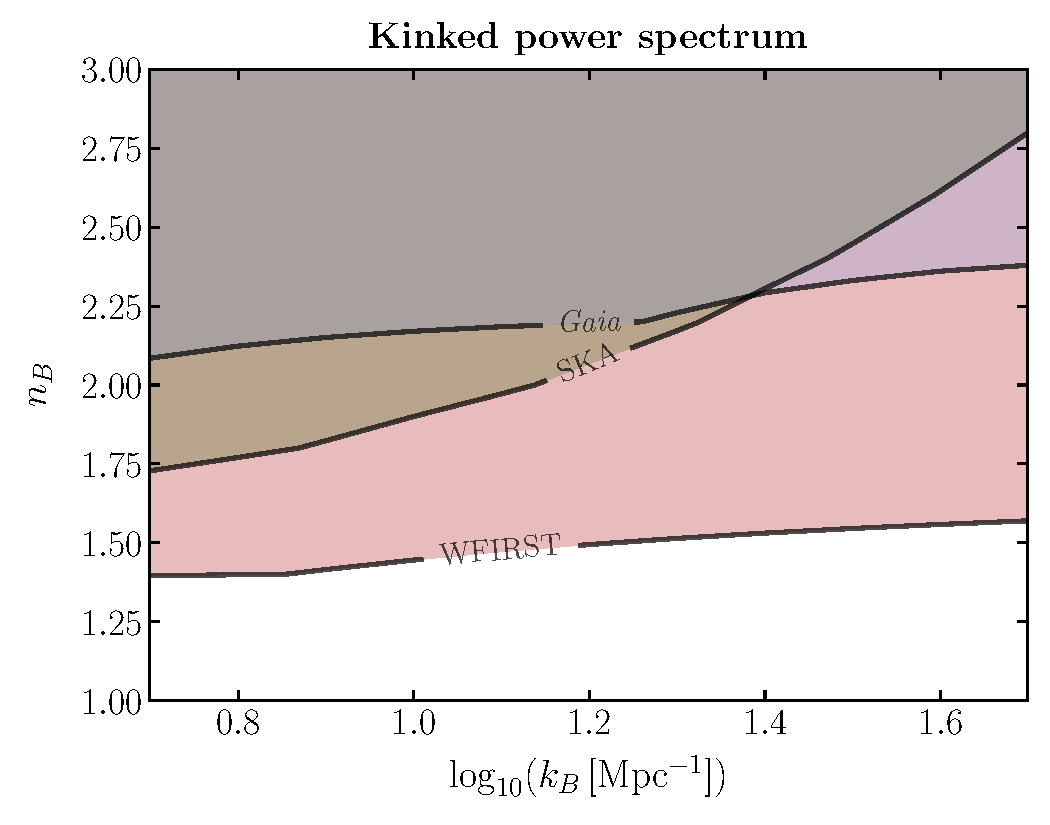
\includegraphics[width=0.47\textwidth]{plots/kink_PS_sig}
  \caption{95\% confidence interval sensitivity forecasts on scenarios with a kink in the power spectrum parameterized by the break location $k_B$ and kink slope $n_B$, assuming a minimum bound substructure mass of $10\,\mathrm M_\odot$. Shown are sensitivities achievable using quasar proper motion measurements with SKA, as well as observations of Galactic stellar proper motion accelerations by WFIRST and (end-of-mission) \Gaia.}
  \label{fig:kink_ps}
\end{figure}

\section{Signal discriminants and further prospects}
\label{sec:handles}

\subsection{Toroidal modes as a control region}

As described in Sec.~\ref{sec:formalism}, since it is sourced from the gradient of the lensing potential, the signal is expected to exclusively populate the poloidal component of the power spectrum decomposition. The noise, on the other hand, is expect to contribute to both the poloidal as well as toroidal modes. The toroidal power spectrum can thus be used as a control region to calibrate the noise.

\subsection{Directional asymmetry}

\begin{figure*}[!htbp]
  \centering
  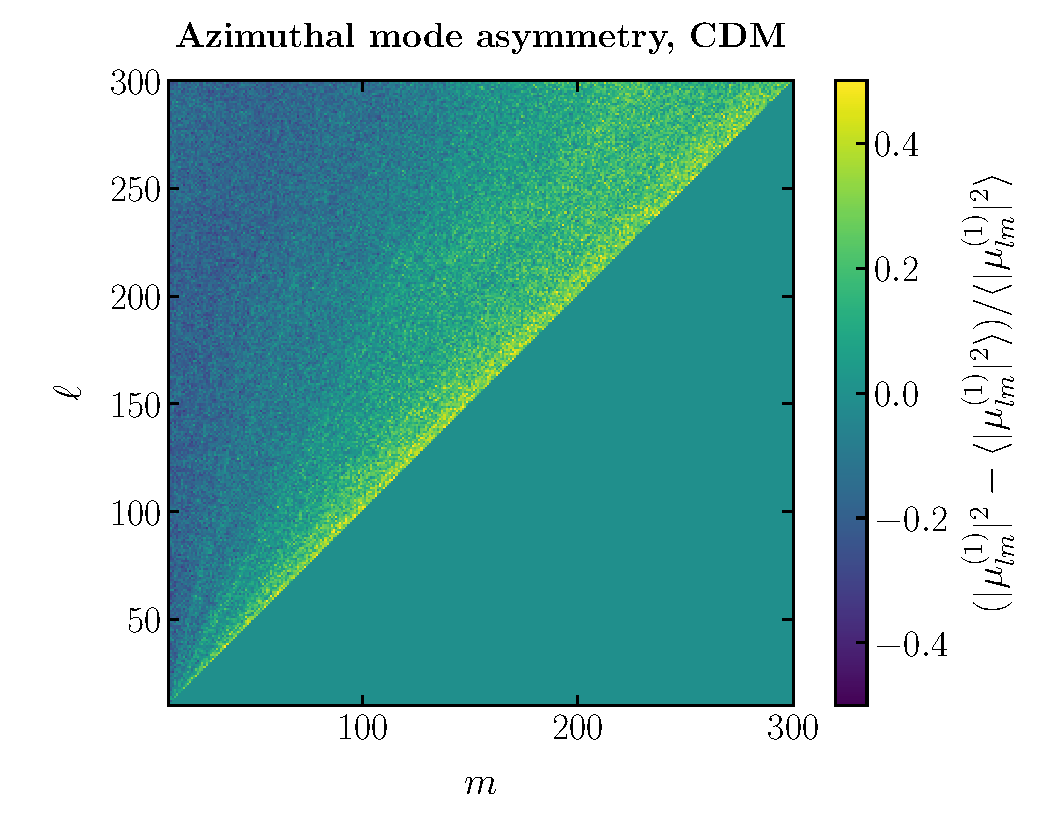
\includegraphics[width=0.47\textwidth]{plots/m_asymm_1}
  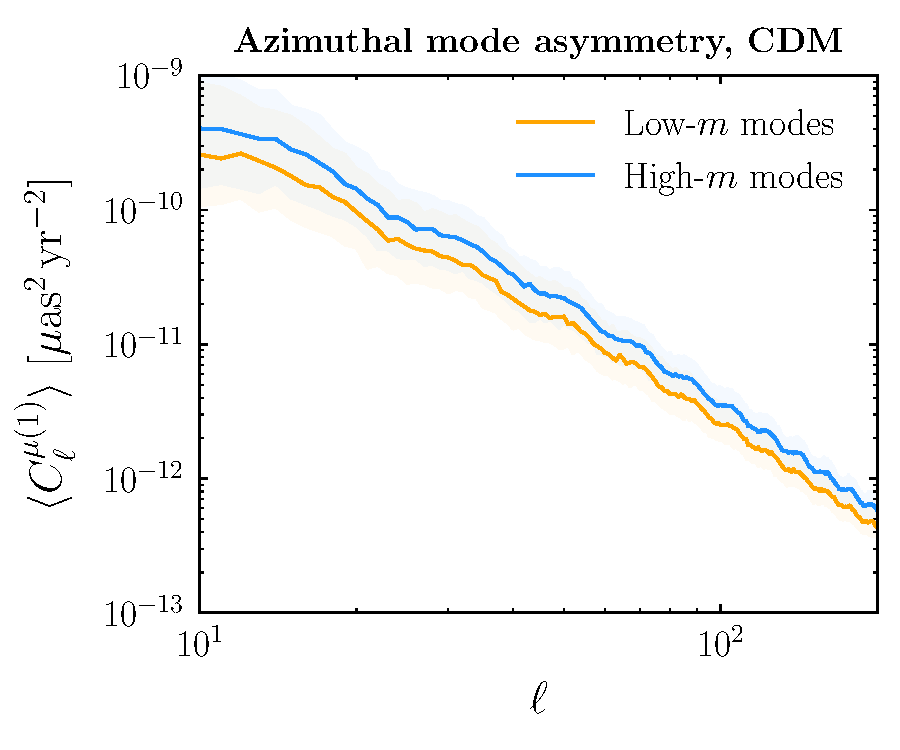
\includegraphics[width=0.45\textwidth]{plots/m_asymm_2}
  \caption{The magnitude of azimuthal asymmetry estimated from simulations for the fiducial CDM setup. (Left) Fractional asymmetry in the power spectrum coefficients $|\mu_\ellm^{(1)}|^2$ averaged over 200 realizations. (Right) High- and low-$m$ components of the power variance evaluated as in Eq.~\ref{eq:asymm}. Bands indicate the middle 50\% containment obtained over the 200 realizations.  $\mathcal{O}(1)$ variation is seen, with larger values with increasing $|m|$ for a fixed $\ell$.}
  \label{fig:m_asymm}
\end{figure*}

After inserting Eq.~\ref{eq:deflectionpotential} into Eq.~\ref{eq:harmdecomposition}, and integrating by parts, and using $\vect{\nabla}_{\vect{\theta}}^2 Y_{\ell m} = - \ell (\ell + 1) Y_{\ell m}$ and Eq.~\ref{eq:PsiPhidef}, we find that for a single lens:
\begin{align}
\mu_{\ell m}^{(1)} = - \frac{\ell (\ell + 1)}{D_l} \int \dd \Omega \, \psi(\vect{\beta}) \vect{v} \cdot \vect{\Psi}_{\ell m}^*.
\end{align}
Due to the Sun's motion around the Galactic center, the probability distribution $f(\vect{v})$ for the effective lens velocity is asymmetric, with higher magnitudes expected for velocity components in the galactic longitude direction than in the galactic latitude direction. This will typically lead to an asymmetry in the expected power at different $m$ values at fixed $\ell$, because the high-$|m|$ (low-$|m|$) modes of $\vect{\Psi}_{\ell m}$ are preferentially oriented along the galactic longitude (latitude) direction. For an isotropically distributed and homogeneous lens population, the signal $\langle |\mu_{\ell m}^{(1)}|^2 \rangle$ will therefore be an \emph{increasing} function of $|m|/\ell$ at fixed $\ell$.

For general lens populations with 3D number density distribution $n(\vect{\theta}_l,D_l)$
\begin{align}
\frac{\langle |\mu_{\ell m'}^{(1)}|^2 \rangle}{\langle |\mu_{\ell m''}^{(1)}|^2 \rangle} = 
\end{align}

The magnitude of the directional asymmetry can be estimated directly from simulations. Figure~\ref{fig:m_asymm} (left) shows the gradually increasing power $|\mu_\ellm|^2$ in the toroidal velocity component with increasing $m$ at a given $\ell$, obtained from 100 simulations of our fiducial CDM-inspired subhalo configuration. This is also illustrated in the right panel of Figure~\ref{fig:m_asymm} (right), where the angular power variance is constructed separately for the low- and high-$m$ components as 
\begin{align}
 C_{\ell,\mathrm{low-}m}^{(1)} &=  \left\langle \sum_{m = 0}^{\mathrm{floor}(\ell_\mathrm{max}/2)} \left| \mu_{\ell m}^{(1)} \right|^2\right\rangle \nonumber \\
 C_{\ell,\mathrm{high-}m}^{(1)} &= \left\langle\sum_{m = {\mathrm{floor}(\ell_\mathrm{max}/2)}}^{\ell_\mathrm{max}} \left| \mu_{\ell m}^{(1)} \right|^2\right\rangle. \label{eq:asymm}
\end{align}
This $\mathcal{O}(1)$ azimuthal asymmetry can be used as a handle to discriminate the signal from the noise, since the latter is expected to contribute uniformly across the $m$-components of the power spectrum coefficients.

% \subsection{Further Prospects}
% \label{sec:prospects}

\section{Conclusions}
\label{sec:conclusions}

Astrometry --- the precise measurement of the positions and motions of celestial bodies --- offers a promising avenue to probe the nature of dark matter through its induced lensing effects. In this paper, we have introduced a novel method to systematically leverage the measured correlated pattern of motions (transverse velocities and accelerations) induced by a population of Galactic subhalos on celestial objects using the formalism of angular two-point correlation functions (angular power spectra). We have shown how to calculate the signal power spectrum for a population of lenses characterized by arbitrary population properties (\emph{e.g.}, distribution of masses and positions) and internal characteristics (\emph{e.g.,} internal profiles). Astrometric datasets deliverable by near-future surveys like SKA and WFIRST will be able to probe a range of well-motivated scenarios such as cold dark matter and scalar field dark matter. Additionally, measurements by the ongoing \emph{Gaia} mission will already be able to probe new parameter space characteristic of enhanced primordial fluctuations on small scales.

Two-point correlations efficiently capture the statistical properties of a map in the limit of the underlying signal being a Gaussian random field. This is true to very good degree for the CMB, for example, with very tight limits on the overall non-Gaussianity, and the decomposition to spherical harmonics comes with little loss of information. Our signal of interest however is highly non-Gaussian, as is apparent from Fig.~\ref{fig:population_maps}, and the spherical harmonic decomposition discards potentially large amounts of information. Methods based on higher-order statistics \emph{e.g.}, bispectra and image processing technique \emph{e.g.}, convolutional filters can leverage additional information in the substructure signal beyond two-point correlations. We leave the study of 

All results and figures presented in this study can be reproduced using the code at \url{https://github.com/smsharma/Lensing-PowerSpectra} \href{https://github.com/smsharma/Lensing-PowerSpectra}{\faGithub}. A link below each figure (\faFileCodeO) provides the python code with which it was generated.

\clearpage
\section*{Acknowledgements}
We thank L.~Chang and D.~Finkbeiner for useful conversations. SM is partially supported by the NSF CAREER grant PHY-1554858 and NSF grant PHY-1620727. This work made use of the NYU IT High Performance Computing resources, services, and staff expertise.
% This research has made use of NASA's Astrophysics Data System.
 This research made use of the \texttt{astropy}~\cite{2013A&A...558A..33A,2018AJ....156..123A}, \texttt{CLASS}~\cite{Blas:2011rf}, \texttt{COLOSSUS}~\cite{2018ApJS..239...35D}, \texttt{healpy}~\cite{2005ApJ...622..759G}, \texttt{IPython}~\cite{PER-GRA:2007}, Mathematica~\cite{Mathematica}, \texttt{matplotlib}~\cite{Hunter:2007}, \texttt{mpmath}~\cite{mpmath}, \texttt{NumPy}~\cite{numpy:2011}, \texttt{pandas}~\cite{pandas:2010} and \texttt{SciPy}~\cite{Jones:2001ab} software packages. 

%\clearpage
\appendix 

\section{Derivation of equations}
\label{app:derivations}

\subsection{Velocity and acceleration power spectra}
In this appendix, we derive the formulae of Eqs.~\ref{eq:pspec_mu} and \ref{eq:pspec_alpha}. It is sufficient to calculate the induced $\mu_{\ell m}^{(1)}$ of a single lens at some distance $D_l$ and enclosed mass function $M(b)$ at a conveniently chosen location and velocity direction $\hat{v}_l$, as the contributions to $C^{\mu(1)}_\ell$ are additive among the lenses, and independent of location/direction by rotational invariance.

The first time derivative of the lensing deflection potential from a single lens is:
\begin{align}
\frac{\dd}{\dd t} \psi = \frac{4G_N M(\beta D_l)}{\beta D_l^2}(\hat{\vect{\beta}} \cdot {\vect{v}}_l ).
\end{align}
Using $\vect{\nabla}_{\vect{\theta}}^2 Y_{\ell m} = -\ell(\ell+1)Y_{\ell m}$ and integration by parts of Eq.~\ref{eq:harmdecomposition}, we find:
\begin{align}
\mu_{\ell m}^{(1)} = \sqrt{\ell(\ell+1)}\int \dd\Omega\, \left(\frac{\dd}{\dd t} \psi(\vect{\theta})\right) Y_{\ellm}^*(\vect{\theta}) \label{eq:muperlens1}
\end{align}
We can evaluate this expression for a lens on the celestial north pole, which implies $\vect{\theta} = \vect{\beta}$, moving with a transverse velocity vector specified by $\vect{v}_l \cdot \hat{\vect{\theta}}  = v_l \cos \phi$.
That allows us to write Eq.~\ref{eq:muperlens1} as:
\begin{align}
\mu_{\ell m}^{(1)} &= \frac{4 G_N v_l}{D_l^2} \sqrt{\ell(\ell+1)}\label{eq:muNP}\\
&\phantom{=}\times \int_0^\pi \dd \theta \, \int_0^{2\pi} \dd \phi \, \cos\phi  \frac{\sin \theta}{\theta} M(\theta D_l) Y^*_{\ell m}(\theta,\phi) \nonumber\\
&\simeq \frac{G_N v_l}{D_l^2} \ell \sqrt{8\pi \ell}\left[\delta_{m,-1}-\delta_{m,1}\right]\int_0^\infty \dd \theta \, M(\theta D_l) J_1(\ell \theta)\nonumber
\end{align}
To get to the final line, we made use of the approximation $P_\ell^m(\cos\theta) \simeq (-1)^m \ell^m J_m(\ell \theta)$ valid for $\theta \ll 1$ (but potentially large $\ell \theta$), and kept only the leading term in the  $1/\ell$ expansion. 

We can similarly find the acceleration power spectrum by computing the amplitudes
\begin{align}
\alpha_{\ell m}^{(1)} = \sqrt{\ell(\ell+1)}\int \dd\Omega\, \left(\frac{\dd^2}{\dd t^2} \psi(\vect{\theta})\right) Y_{\ellm}^*(\vect{\theta}), \label{eq:alphaperlens1}
\end{align}
using the fact that
\begin{align}
\frac{\dd^2}{\dd t^2} \psi &= \frac{4G_N}{D_l^3} \bigg\lbrace\frac{(\hat{\vect{\beta}} \cdot {\vect{v}}_l)^2}{\beta}  \partial_\beta M(\beta D_l) \\
&\phantom{=\frac{4G_N}{D_l^3} \bigg\lbrace} + \frac{v_l^2 - 2 (\hat{\vect{\beta}} \cdot {\vect{v}}_l)^2 }{\beta^2}M(\beta D_l)\bigg\rbrace. \nonumber
\end{align}
Evaluating at the north pole as in Eq.~\ref{eq:muNP} yields
\begin{align}
\alpha_{\ell m}^{(1)}  = \frac{G_N v_l^2}{D_l^3} \ell^2 \sqrt{8\pi \ell}\left[\delta_{m,0}-\frac{\delta_{|m|,2}}{2} \right]\int_0^\infty \dd \theta \, M(\theta D_l) J_1(\ell \theta),\label{eq:alphaNP}
\end{align}
where we integrated by parts (and assumed $M(b)\to 0$ as $b\to 0$) to cast the acceleration amplitude in a similar form as the velocity amplitude. We note that the dependence on the enclosed mass function in Eqs.~\ref{eq:muNP} and \ref{eq:alphaNP} is identical, giving the simple scaling relation between the corresponding power spectra stated in Eq.~\ref{eq:pspec_alpha}.

\subsection{Flat-sky velocity power spectrum}

\subsection{Power spectrum for ultralight scalar dark matter perturbations}

% \subsection{Derivation of transfer function}
% Define $y \equiv a / a_\mathrm{eq}$, $u_k \equiv k/\sqrt{3}a H$, and a dimensionless wavenumber:
% \begin{align}
% \tilde{k} \equiv \frac{k/a_\mathrm{eq}}{H_\mathrm{eq}}
% \end{align}
% A primordial curvature perturbation $\Phi_{0,k}$ with wavenumber $k$ that enters the horizon long before matter-radiation equality, i.e.~$\tilde{k} \gg 1$, has a covariant density perturbation $\Delta_k$ solution as a function of time $u_k$ 
% \begin{align}
% \Delta_k &= - 9 \Phi_{0,k} \bigg[ \frac{\sin(u_k)}{u_k} + \frac{\cos(u_k)-1}{u_k^2}\\
% &\phantom{= - 9 \Phi_{0,k} \bigg[} + \ln(u_k) - \mathrm{Ci}(u_k) + \gamma_\mathrm{E} - \frac{1}{2} \bigg] \nonumber \\
% &\simeq - 9 \Phi_{0,k} \bigg[ \ln(\tilde{k} y) + \gamma_\mathrm{E} - \frac{1}{2} + \frac{1}{2} \ln \frac{2}{3} \bigg]. \label{eq:Deltasol}
% \end{align}
% The first equation above is valid for $y \ll 1$, while the last line makes the further approximation that the mode is well within the horizon $y \gg 1/\tilde{k}$.
% The evolution of subhorizon density perturbations is well-described by the Newtonian differential equation:
% \begin{align}
% (1+y) \delta_k'' + \left(\frac{1}{y} + \frac{3}{2} \right) \delta_k' - \frac{3}{2y} \delta_k = 0
% \end{align}
% which is solved by
% \begin{align}
% \delta_k(y) &= c_{1,k} \left( \frac{2}{3} + y\right) \label{eq:deltasol} \\
% &\phantom{=} + c_{2,k} \frac{3}{2} \left[3 \sqrt{1+y} - (2 + 3 y) \mathrm{arctanh}(\sqrt{1+y}) \right] \nonumber
% \end{align}
% The leading pieces in the Taylor expansion of Eq.~\ref{eq:deltasol} in the regime $y\ll 1$ also yield a $\ln(y)$ term plus a constant; matching to Eq.~\ref{eq:Deltasol} then fixes the coefficients to be $c_{2,k} = -6 \Phi_{0,k}$ and $c_{1,k} = -(27 \Phi_{0,k}/4)[-7+\gamma_\mathrm{E} - 2i \pi + \ln(32/3)+2\ln(\tilde{k})]$. Note that we now have a closed-form solution for density perturbations at all times in a Universe with dark matter and radiation only, and therefore also the transfer function:
% \begin{align}
% D(k,a) \equiv \frac{\delta_k(y)}{\Phi_{0,k}}. \label{eq:transferfun}
% \end{align}
% We are ignoring 20\%-level corrections due to baryonic matter, and even smaller corrections due to the presence of the vacuum energy, which plays a subdominant role for $a \lesssim 1/2$, the regime of interest.

% \blue{should probably do another stage of matching to include the cc today}

% We note that the above approach only works for scales which enter the horizon much before matter-radiation equality $\tilde{k}$, such that the regime $1/\tilde{k} \ll y \ll 1$ exists parametrically. We are primarily interested in structures with scale masses $\lesssim 10^{10} M_\odot$, for which it is indeed true that $\tilde{k} \gtrsim 10^{3}$, as the halo scale mass versus wavenumber correspondence is parametrically:
% \begin{align}
% M_s \sim \frac{4\pi}{3} \rho \left(\frac{\pi}{k}\right)^3 \approx 6 \times 10^9 M_\odot \left( \frac{10^3}{\tilde{k}} \right)^3.
% \end{align}
% We expect the matching procedure during radiation domination to contribute a fractional error in $\delta_k(y)$ at late times of order $2/\sqrt{\tilde{k}}$, at the 10\% level at worst for the scales under consideration.


\section{Fisher forecasting formalism}
\label{sec:fisher}

Assuming that the vector spherical harmonic coefficients $\mu_\ellm^{\alpha}$ are Gaussian-distributed with a (cross-)variance given by the power spectra $C_\ell^{\alpha\beta}$~\footnote{Here, $\alpha$ and $\beta$ could refer to, for example, toroidal or poloidal modes, proper motion or proper motion acceleration spectra, high/low-$m$ modes.} (Eq~\ref{}), it can readily be shown that (see, \emph{e.g.}, Ref.~\cite{}), up to a constant factor,  the log-likelihood for a given realization of the harmonic coefficients is given by 
\begin{equation}
\ln \mathcal L = -\frac{1}{2}\left[\sum_{\ell,m}\vect{\mu}_\ellm^T\mathsf C_\ell^{-1}\vect{\mu}_\ellm - \ln(\det[\mathsf C_\ell])\right]
\label{eq:like}
\end{equation}
where the individual harmonic coefficients are written as vectors $[\vect{\mu}_\ellm]_\alpha \equiv \mu_\ellm^\alpha$ and the cross-spectra are written as matrices $[\mathsf C_\ell]_{\alpha\beta}\equiv C_\ell^{\alpha\beta}$. We wish to produce sensitivity forecasts for how well a given signal configuration, parameterized by a set of parameters ${\theta_i}$, can be measured given an experimental configuration. For this, we appeal to the Fisher matrix formalism. Here, the likelihood Eq.~\ref{eq:like} is approximated by a Gaussian series around a set of fiducial parameters ${\overline{\theta}_i}$,
\begin{equation}
\ln \mathcal L = -\frac{1}{2}\sum_{i,j}(\theta_i - \overline{\theta}_i)\,F_{ij}\,(\theta_j - \overline{\theta}_j),
\end{equation}
where we define the Fisher matrix $F_{ij}\equiv\langle\partial^2\mathcal{L}/\partial\theta_i\partial\theta_j\rangle$. The covariance matrix $C_{ij}\equiv \langle(\theta_i - \overline\theta_i)(\theta_j - \overline\theta_j)\rangle$ can be approximated as the inverse of the Fisher matrix. For our likelihood Eq.~\ref{eq:like} it can be shown that
\begin{equation}
F_{ij} = f_\mathrm{sky}\sum_{\ell=\ell_\mathrm{min}}^{\ell_\mathrm{max}}\frac{(2\ell + 1)}{2}\mathrm{Tr}\left[(\partial_i\mathsf C_\ell)\mathsf C_\ell^{-1}\partial_j\mathsf C_\ell)\mathsf C_\ell^{-1}\right]
\label{eq:fisher}
\end{equation}
with $\partial_j\equiv\partial/\partial\theta_i$ and where $f_\mathrm{sky}$ accounts for the incomplete sky-coverage fraction of a given observation.

The observed coefficients are modeled as the sum of the signal (correlated induced motions) and noise (instrumental/shot noise): $\vect{\mu}_\ellm =\vect{\mu}_\ellm^S + \vect{\mu}_\ellm^N$. Assuming the signal and noise are uncorrelated, we have $\mathsf{C}_\ell = \mathsf{C}_\ell^S + \mathsf{N}_\ell$, where $\mathsf{C}_\ell^S$ are the signal spectra calculated with Eq.~\ref{eqn:popcell} and $\mathsf{N}_\ell$ are the noise spectra which depend on the particular observation.

The derivatives required by Eq.~\ref{eq:fisher} are calculated with central finite differences,
\begin{equation}
\partial_if = \frac{f(\theta_i + \delta\theta_i) - f(\theta_i - \delta\theta_i)}{2\delta\theta_i} + \mathcal{O}(\delta\theta_i^3),
\end{equation}
where we make sure that the results are stable to the choices of ${\delta\theta_i}$.

It will be useful to impose priors on certain parameters in order to mitigate degeneracies. Assuming a Gaussian prior on parameter $\theta_i$, in the Fisher formalism this can easily be done by adding the inverse covariance to the corresponding term in the Fisher matrix, $F_{ii} \rightarrow F_{ii} + \sigma_i^{-2}$.

In this study, we model the instrumental component as white (scale-invariant) noise, democratically contributing at each mode. In particular, for proper motion noise $\sigma_\mu$ and number of quasars sampled $N_q$, the noise contribution per mode is $N_\ell = \sigma_\mu^2/N_q$

\section{Constructing a velocity power spectrum estimator}

\SMS{Just copied this out from @kvt notes...}

\subsection{Setup}
Vector data on the sphere $d_{j\alpha} = s_{j\alpha} + n_{j\alpha}$ composed of a signal $s$ and noise $n$. Sphere is tessellated in equal-area pixels denoted by $j = 1, \dots, J$. The greek index $\alpha = 1,2$ runs over the two vector components in the colatitude $\theta$ and longitude $\varphi$ directions. Using spherical harmonics defined as
\begin{align}
Y_{\ell m}(\theta, \varphi) = (-1)^m \sqrt{\frac{2\ell + 1}{4\pi}\frac{(\ell - m)!}{(\ell + m)!}} P_{\ell m}(\cos \theta) e^{i m \varphi}
\end{align}
where $P_{\ell m}$ are the associated Legendre polynomials without the Condon-Shortley phase.  With $\nabla = \hat{\vect{\theta}} \partial_\theta +  \hat{\vect{\varphi}} (\sin \theta)^{-1} \partial_\varphi$, define vector spherical harmonics as
\begin{widetext}
\begin{align}
\vect{\Psi}_{\ell m} &\equiv \frac{\nabla Y_{\ell m} }{\sqrt{\ell (\ell + 1)}}; \quad \vect{\Phi}_{\ell m} = \hat{\vect{r}} \times \vect{\Psi}_{\ell m}\\
\vect{\Psi}_{\ell m} &= \frac{-1}{\sin \theta} \frac{1}{\sqrt{\ell (\ell + 1) }} \left\lbrace \hat{\vect{\theta}} \left[ (\ell+1) \sqrt{\frac{(\ell - m)(\ell + m)}{(2\ell - 1)(2 \ell + 1)}} Y_{\ell-1,m} - \ell   \sqrt{\frac{(\ell - m+1)(\ell + m+1)}{(2\ell +3)(2 \ell + 1)}} Y_{\ell+1,m} \right] + \hat{\vect{\varphi}} i m Y_{\ell m} \right\rbrace
\end{align}
\end{widetext}
with a similar formula for $\vect{\Phi}_{\ell m}$. Normalization is such that $\int \vect{\Psi}_{\ell m} \cdot \vect{\Psi}_{\ell' m'}  d\Omega = \delta_{\ell \ell'} \delta_{m m'}$, likewise for $\vect{\Phi}$, cross-term integrals always zero. 
Define shorthand $Y^{\ell m}_j \equiv Y_{\ell m}(\theta_j, \varphi_j)$, $\Psi^{\ell m}_{j \alpha} \equiv \Psi_{\ell m, \alpha}(\theta_j, \varphi_j)$, etc.

Can write any field, e.g.~the signal, as
\begin{widetext}
\begin{align}
s_{j\alpha} = \sum_{\ell m} s_{\ell m}^{(1)} \Psi^{\ell m}_{j \alpha} +  s_{\ell m}^{(2)} \Phi^{\ell m}_{j \alpha}; \quad s_{\ell m}^{(1)} = \frac{4\pi}{J} \sum_{j \alpha} s_{j\alpha} \Psi^{\ell m *}_{j \alpha}; \quad s_{\ell m}^{(2)} = \frac{4\pi}{J} \sum_{j \alpha} s_{j\alpha} \Phi^{\ell m *}_{j \alpha}
\end{align}
\end{widetext}

Expect signal only in $s_{\ell m}^{(1)}$, not in $s_{\ell m}^{(2)}$.

Covariance matrix of data, with uncorrelated signal and noise:
\begin{align}
C_{i\alpha j \beta} = \langle d_{i \alpha} d_{j \beta} \rangle = \langle s_{i \alpha} s_{j \beta} \rangle + \langle n_{i \alpha} n_{j \beta} \rangle \equiv S_{i \alpha j \beta} + N_{i \alpha j \beta}
\end{align}
Express signal covariance matrix in terms of its power spectrum $S$ and response matrices $P$:
\begin{widetext}
\begin{align}
S_{i \alpha j \beta} = \sum_{\ell m} S^{(1)}_{\ell m} P_{i \alpha j \beta}^{(1) \ell m } + S^{(2)}_{\ell m} P_{i \alpha j \beta}^{(2) \ell m }; \quad \langle s^{(1)}_{\ell m} s^{(1)*}_{\ell m} \rangle \equiv S^{(1)}_{\ell m} \delta_{\ell \ell'} \delta_{m m'}; \quad P_{i \alpha j \beta}^{(1) \ell m } \equiv \Psi_{i \alpha}^{\ell m} \Psi_{j \beta}^{\ell m *}
\end{align}
\end{widetext}

We assume the noise covariance matrix is known; for simplicity, can assume it is uncorrelated between pixels (for now) and isotropic in direction:
\begin{align}
N_{i \alpha j \beta} = N_i \delta_{ij} \delta_{\alpha \beta} \quad \text{(no sum over $i$)} \label{eq:Ndiagonal}
\end{align}

\subsection{Quadratic likelihood estimator}
Likelihood:
\begin{align}
\mathcal{L} = \frac{\exp\left\lbrace -\frac{1}{2} d_{i \alpha} \Cinv_{i \alpha j \beta} d_{j \beta} \right\rbrace}{(2\pi)^J \sqrt{\det C}}
\end{align}
Log likelihood $L \equiv - 2 \ln \mathcal{L}$. We are interested in finding the signal power spectrum $S^{(1)}_{\ell m}$ and thus the correct $C$ covariance matrix that minimizes the log likelihood. (Can repeat same analysis for $S^{(2)}_{\ell m}$ which should be control channel.)

First derivative:
\begin{align}
\frac{\partial L}{\partial S^{(1)}_{\ell m}} = \Cinv_{i \alpha j \beta} P^{(1) \ell m}_{j \beta i \alpha} - d_{a \alpha} \Cinv_{a \alpha b \beta} P^{(1) \ell m}_{b \beta c \gamma} \Cinv_{c \gamma e \epsilon} d_{e \epsilon}
\end{align}
Can show that $\langle {\partial L}/{\partial S^{(1)}_{\ell m}} \rangle = 0$ if $C = \langle d d \rangle$. After calculating the Hessian $ {\partial^2 L}/{\partial S^{(1)}_{\ell m} \partial S^{(1)}_{\ell' m'}}$, can devise an iterative procedure based on the Newton-Raphson method that finds a local minimum of $L$, as in Ref.~\cite{dahlen2008spectral}. \blue{[Too lazy to write this out.]} If the global minimum $\bar{S}^{(1)}_{\ell m}$ is found, then this maximum-likelihood estimator $\hat{S}^{(1)}_{\ell m} = \bar{S}^{(1)}_{\ell m}$ is guaranteed to be the optimal unbiased estimator:
\begin{widetext}
\begin{align}
\hat{S}^{(1)}_{\ell m} &= d_{i\alpha} Z^{(1) \ell m}_{i\alpha j \beta} d_{j \beta} - N_{i \alpha j \beta} Z^{(1) \ell m}_{j \beta i\alpha}; \\
Z^{(1) \ell m}_{i \alpha j \beta} &= \frac{1}{2} \sum_{\ell' m'} (F_{(1)}^{-1})_{\ell m \ell' m'} \Cinv_{i \alpha i' \alpha'} P^{(1) \ell' m'}_{i' \alpha' j' \beta'} \Cinv_{j' \beta' j \beta} \\
F^{(1)}_{\ell m \ell' m'} &= \frac{1}{2} \Cinv_{a \alpha b \beta} P^{(1) \ell m}_{b \beta c \gamma} \Cinv_{c \gamma e \epsilon} P^{(1) \ell' m'}_{e \epsilon a \alpha} \\
\text{Cov}\left\lbrace \hat{S}^{(1)}_{\ell m} \hat{S}^{(1)}_{\ell' m'} \right\rbrace &= (F_{(1)}^{-1})_{\ell m \ell' m'}
\end{align}
\end{widetext}

Note that the last equation is the covariance matrix of the estimator, thus providing error estimates on the measurement.
In the above, $Z$ and the Fisher matrix $F$ are to be evaluated at $\bar{S}$ on the RHS of the $\hat{S}$ formula, which is why an iterative procedure is needed. However, in the limit where the signal power is small compared to the noise power $S \ll N$ in any one (spatial or spectral) bin, which is the regime of interest, we can make the approximation $C \simeq N$ at the cost of slightly biasing the estimator by a fractional amount of $S/N$. In this case, no iteration is needed. If we further assume that $N$ is diagonal as in Eq.~\ref{eq:Ndiagonal}, we find:
\begin{widetext}
\begin{align}
\hat{S}^{(1)}_{\ell m} &= \frac{1}{2} \sum_{\ell' m'} (F_{(1)}^{-1})_{\ell m \ell' m'} \left[\sum_{i j \alpha \beta}  \frac{ d_{i \alpha} d_{j \beta}}{N_i N_j} P^{(1)\ell m}_{i \alpha j \beta} - \sum_{i \alpha}  \frac{P^{(1)\ell m}_{i \alpha i \alpha}}{N_i} \right] \\
F^{(1)}_{\ell m \ell' m'} &= \frac{1}{2} \sum_{i j \alpha \beta} \frac{P^{(1)\ell m}_{i \alpha j \beta} P^{(1)\ell' m'}_{j \beta i \alpha}}{N_i N_j}
\end{align}
\end{widetext}


If the noise were the same in each pixel, $N_i = \sigma^2~ \forall i$, then we would have a diagonal Fisher matrix $F^{(1)}_{\ell m \ell' m'} = (J/2\sigma^4)\delta_{\ell \ell'} \delta_{m m'}$ and an even simpler estimator: $\hat{S}^{(1)}_{\ell m} = d_{i \alpha} d_{j \beta} P^{(1)\ell m}_{i \alpha j \beta} - \sigma^2$. Empty pixels $d_i$ carry no information; it can be seen from the likelihood or its estimator that not summing over empty pixels $d_i$ is equivalent to taking their noise to be infinite $N_i = \infty$.

Define $(\ell m)$ Fourier amplitude of $f^{\ell' m'}_i$ to be $f_{\ell m}^{\ell' m'}$. 
\begin{widetext}
\begin{align}
P^{(1) \ell m}_{i\alpha j \beta} = \Psi^{\ell m}_{i\alpha} \Psi^{\ell m *}_{j \beta}; \qquad 
\Psi^{\ell m}_{i \alpha} = \frac{-1}{\sin \theta_i} \left\lbrace \delta_{\alpha 1} \left[ c^{\ell m}_1 Y^{\ell-1, m}_i + c^{\ell m}_2 Y^{\ell+1, m}_i \right] + \delta_{\alpha 2} c^{\ell m}_3 Y^{\ell m}_i \right\rbrace 
\end{align}
\end{widetext}

\begin{widetext}
\begin{align}
c^{\ell m}_1 &= \frac{\ell + 1}{\sqrt{\ell(\ell+1)}} \sqrt{\frac{(\ell - m)(\ell + m)}{(2\ell -1)(2\ell +1)}}; \quad
c^{\ell m}_2 = \frac{-\ell}{\sqrt{\ell(\ell+1)}} \sqrt{\frac{(\ell - m+1)(\ell + m+1)}{(2\ell +3)(2\ell +1)}}; \quad
c^{\ell m}_3 = \frac{i m}{\sqrt{\ell(\ell+1)}} \\
A^{\ell m}_i &= \frac{1}{N_i \sin \theta_i} \left( c^{\ell m}_1 Y^{\ell-1,m}_i + c^{\ell m}_2 Y^{\ell+1,m}_i \right); \qquad 
B^{\ell m}_i = \frac{1}{N_i \sin \theta_i} c^{\ell m}_3 Y^{\ell m}_i\\ 
F_{\ell m \ell' m'} &=  \big\lbrace c^{\ell' m'}_1 A^{\ell m}_{\ell'-1,m'} + c^{\ell' m'}_2 A^{\ell m}_{\ell'+1,m'} - c^{\ell' m'}_3 B^{\ell m}_{\ell' m'} \big\rbrace \big\lbrace \text{(transpose)} \big\rbrace
\end{align}
\end{widetext}

First compute $A^{\ell m}_{\ell' m'}$ and $B^{\ell m}_{\ell' m'}$ matrices, and then construct Fisher matrix.

\subsection{Spectral binning}
The maximum likelihood estimator requires the inverse of the Fisher matrix, which may not exist if the data are too sparse and $\ell_\text{max}$ is too large. Since we are not interested in the power in any one mode, but rather in the gross behavior, we would collect the power spectrum into logarithmic bins in $\ell$, and a high-$|m|$ bin, and a low-$|m|$ bin anyway.

Non-overlapping spectral bins $B$. Binning by $m$ could be e.g.~$B+ = \lbrace m : |m|\le\text{floor}(\ell/2)\rbrace$ and $B- = \lbrace m : \text{floor}(\ell/2) < |m|\le \ell \rbrace$.  Compute ``band averages'':
\begin{align}
S^{(1)}_B = \sum_{\ell m} W_{B \ell m} S^{(1)}_{\ell m},
\end{align}
with weight matrices $W_{B \ell m}$ that have many fewer rows than columns and which satisfy $\sum_{\ell m} W_{B \ell m} = 1$. We suppose that the power spectrum can be adequately approximated by the coarse-grained $S_l^{(1)\dagger}$:
\begin{align}
S^{(1)\dagger}_{\ell m} = \sum_B W_{\ell m B}^\dagger S_B^{(1)}
\end{align}
where $W_{\ell m B}^\dagger$ is the pseudo-inverse
\begin{align}
W_{\ell m B}^\dagger = \sum_{B'} W_{B \ell m} \left( \sum_{\ell' m'} W_{B' \ell' m'} W_{B \ell' m'} \right)^{-1}
\end{align}

All formulas for $S_B$, $Z_{B B'}$, and $F_{BB'}$ are the same as in the previous section with the replacements $\ell m \leftrightarrow B$ and using the weighted response matrices:
\begin{align}
P^{(1)B}_{i\alpha j \beta} = \sum_{\ell m} P^{(1)\ell m}_{i\alpha j \beta} W^\dagger_{\ell m B}.
\end{align}

% \bibliographystyle{aasjournal}
\bibliographystyle{aasjournal-mod}
% \bibliographystyle{apj}

\bibliography{lenspower}

\end{document}
